\def\year{2021}\relax
%File: formatting-instructions-latex-2021.tex
%release 2021.1
\documentclass[letterpaper]{article} % DO NOT CHANGE THIS
\usepackage{aaai21}  % DO NOT CHANGE THIS
\usepackage{times}  % DO NOT CHANGE THIS
\usepackage{helvet} % DO NOT CHANGE THIS
\usepackage{courier}  % DO NOT CHANGE THIS
\usepackage[hyphens]{url}  % DO NOT CHANGE THIS
\usepackage{graphicx} % DO NOT CHANGE THIS
\usepackage{amsmath}
\usepackage{booktabs}
\usepackage{amssymb}
\usepackage{mathrsfs}
\usepackage{soul}
\usepackage{amsfonts}
\usepackage{framed}
\usepackage{tikz}
\usetikzlibrary{arrows,shapes.geometric,shapes.arrows}
\usepackage{pgfplots}
\usepackage{amsthm} 
\usepackage[ruled,vlined,linesnumbered]{algorithm2e} 
\usepackage{makecell}
\usepackage{tikz}
\usepackage{comment}
\urlstyle{same}
\usepackage{multirow}
\usepackage{times}
\usepackage{helvet}
\usepackage{courier}
\newtheorem{theorem}{Theorem}
\newtheorem{definition}{Definition}
\newtheorem{observation}{Observation}
\newtheorem{corollary}{Corollary}
\newtheorem{lemma}{Lemma}
\newtheorem{example}{Example}
\newtheorem{conjecture}{Conjecture}
\usepackage[ruled,linesnumbered]{algorithm2e}
\newcommand{\var}{\texttt}
\usepackage{mathtools} % Bonus
\usepackage{lipsum}
\usepackage{csquotes}
\usepackage{verbatim}
\usepackage{array,multirow,graphicx}
\usepackage{url}
\definecolor{Blue}{rgb}{0,0.16,0.90}
\definecolor{Red}{rgb}{0.90,0.16,0}
\definecolor{DarkBlue}{rgb}{0,0.08,0.45}
\definecolor{ChangedColor}{rgb}{0.9,0.08,0}
\definecolor{CommentColor}{rgb}{0.2,0.8,0.2}
\definecolor{ToDoColor}{rgb}{0.1,0.2,1}

\definecolor{verylightgray}{rgb}{0.91,0.91,0.91}

% *** Use this definition of the command to show the meta-info ***
\newcommand{\todo}[1]{\textbf{\color{ToDoColor} TODO: #1}}
%\newcommand{\tal}[1]{\footnote{\textbf{\color{CommentColor} /* #1   (tal)*/}}}
%\newcommand{\liat}[1]{\footnote{\textbf{\color{CommentColor} /* #1   (liat)*/}}}
%\newcommand{\roni}[1]{\footnote{\textbf{\color{CommentColor} /* #1   (roni)*/}}}


\newcommand{\tuple}[1]{\langle#1\rangle}
\newcommand{\generalnote}[1]{#1}
\newcommand{\argmax}{\textit{argmax}}

\usepackage{xspace}

\usepackage{acronym}
\acrodef{SAMD}{Supplier Assignment for Meeting a Deadline}
\newcommand{\samd}{\ac{SAMD}\xspace}

\newcommand{\astar}{\textsc{A*}\xspace}
\newcommand{\cM}{{\cal M}}
\newcommand{\Posp}{\mathit{Pos\mbox{-}p}}
\newcommand{\Negp}{\mathit{Neg\mbox{-}p}}
\newcommand{\sampling}{\textsc{Sampling}\xspace}
\newcommand{\expectation}{\textsc{Expectation}\xspace}
\newcommand{\bnb}{\textsc{B\&B}\xspace}
\newcommand{\closed}{\textsc{Closed}\xspace}
\newcommand{\open}{\textsc{Open}\xspace}
\newcommand{\optapprox}{\textsc{OptApprox}\xspace}
\newcommand{\invoptapprox}{\textsc{InvOptApprox}\xspace}
\newcommand{\appr}{\textsc{Approx}\xspace}
\newcommand{\astarapprox}{\textsc{A*$_\appr$}\xspace}

%
% Add comments in the text
%
\newboolean{showcomments}
\setboolean{showcomments}{true}
%\setboolean{showcomments}{false}

\ifthenelse{\boolean{showcomments}}
  {\newcommand{\nb}[3]{
  {\color{#2}\small\fbox{\bfseries\sffamily\scriptsize#1}}
  {\color{#2}\sffamily\small$\triangleright~$\textit{\small #3}$~\triangleleft$}
  }
  }
  {\newcommand{\nb}[3]{}
  }

\newcommand\Liat[1]{\nb{\textbf{Liat:}}{red}{#1}}
\newcommand\Tal[1]{\nb{\textbf{Tal:}}{green}{#1}}
\newcommand\Roni[1]{\nb{\textbf{Roni:}}{blue}{#1}}
\setcounter{secnumdepth}{2} %May be changed to 1 or 2 if section numbers are desired.
\newcommand{\commentout}[1]{}
\title{Assigning Suppliers to Meet a Deadline }
\commentout{
\author{
    %Authors
    % All authors must be in the same font size and format.
    Written by AAAI Press Staff\textsuperscript{\rm 1}\thanks{With help from the AAAI Publications Committee.}\\
    AAAI Style Contributions by Pater Patel Schneider,
    Sunil Issar,  \\
    J. Scott Penberthy,
    George Ferguson,
    Hans Guesgen,
    Francisco Cruz,
    Marc Pujol-Gonzalez
    \\
}
\affiliations{
    %Afiliations

    \textsuperscript{\rm 1}Association for the Advancement of Artificial Intelligence\\
    %If you have multiple authors and multiple affiliations
    % use superscripts in text and roman font to identify them.
    %For example,

    % Sunil Issar, \textsuperscript{\rm 2}
    % J. Scott Penberthy, \textsuperscript{\rm 3}
    % George Ferguson,\textsuperscript{\rm 4}
    % Hans Guesgen, \textsuperscript{\rm 5}.
    % Note that the comma should be placed BEFORE the superscript for optimum readability

    2275 East Bayshore Road, Suite 160\\
    Palo Alto, California 94303\\
    % email address must be in roman text type, not monospace or sans serif
    publications21@aaai.org

    % See more examples next
}
\iffalse
%Example, Single Author, ->> remove \iffalse,\fi and place them surrounding AAAI title to use it
\title{My Publication Title --- Single Author}
\author {
    % Author
    Author Name \\
}

\affiliations{
    Affiliation \\
    Affiliation Line 2 \\
    name@example.com
}
\fi

\iffalse
%Example, Multiple Authors, ->> remove \iffalse,\fi and place them surrounding AAAI title to use it
\title{My Publication Title --- Multiple Authors}
\author {
    % Authors

        First Author Name,\textsuperscript{\rm 1}
        Second Author Name, \textsuperscript{\rm 2}
        Third Author Name \textsuperscript{\rm 1} \\
}
\affiliations {
    % Affiliations
    \textsuperscript{\rm 1} Affiliation 1 \\
    \textsuperscript{\rm 2} Affiliation 2 \\
    firstAuthor@affiliation1.com, secondAuthor@affilation2.com, thirdAuthor@affiliation1.com
}
\fi
}

\author {\# 4613}

\urlstyle{rm} % DO NOT CHANGE THIS
\def\UrlFont{\rm}  % DO NOT CHANGE THIS
\usepackage{natbib}  % DO NOT CHANGE THIS AND DO NOT ADD ANY OPTIONS TO IT
\usepackage{caption} % DO NOT CHANGE THIS AND DO NOT ADD ANY OPTIONS TO IT
\frenchspacing  % DO NOT CHANGE THIS
\setlength{\pdfpagewidth}{8.5in}  % DO NOT CHANGE THIS
\setlength{\pdfpageheight}{11in}  % DO NOT CHANGE THIS
%\nocopyright
%PDF Info Is REQUIRED.
% For /Author, add all authors within the parentheses, separated by commas. No accents or commands.
% For /Title, add Title in Mixed Case. No accents or commands. Retain the parentheses.
\usepackage{times}
\usepackage{soul}
\usepackage{url}
\usepackage[utf8]{inputenc}
%\usepackage[small]{caption}
%\usepackage{algorithm}
%\usepackage{algorithmic}
%-------------------
%% Farbige Kommentar-Felder
%\usepackage[usenames]{color} % Only used in comment commands
%\usepackage{hyperref}
% /Title ()
% Put your actual complete title (no codes, scripts, shortcuts, or LaTeX commands) within the parentheses in mixed case
% Leave the space between \Title and the beginning parenthesis alone
% /Author ()
% Put your actual complete list of authors (no codes, scripts, shortcuts, or LaTeX commands) within the parentheses in mixed case.
% Each author should be only by a comma. If the name contains accents, remove them. If there are any LaTeX commands,
% remove them.
% DISALLOWED PACKAGES
% \usepackage{authblk} -- This package is specifically forbidden
% \usepackage{balance} -- This package is specifically forbidden
% \usepackage{color (if used in text)
% \usepackage{CJK} -- This package is specifically forbidden
% \usepackage{float} -- This package is specifically forbidden
% \usepackage{flushend} -- This package is specifically forbidden
% \usepackage{fontenc} -- This package is specifically forbidden
% \usepackage{fullpage} -- This package is specifically forbidden
% \usepackage{geometry} -- This package is specifically forbidden
% \usepackage{grffile} -- This package is specifically forbidden
% \usepackage{hyperref} -- This package is specifically forbidden
% \usepackage{navigator} -- This package is specifically forbidden
% (or any other package that embeds links such as navigator or hyperref)
% \indentfirst} -- This package is specifically forbidden
% \layout} -- This package is specifically forbidden
% \multicol} -- This package is specifically forbidden
% \nameref} -- This package is specifically forbidden
% \usepackage{savetrees} -- This package is specifically forbidden
% \usepackage{setspace} -- This package is specifically forbidden
% \usepackage{stfloats} -- This package is specifically forbidden
% \usepackage{tabu} -- This package is specifically forbidden
% \usepackage{titlesec} -- This package is specifically forbidden
% \usepackage{tocbibind} -- This package is specifically forbidden
% \usepackage{ulem} -- This package is specifically forbidden
% \usepackage{wrapfig} -- This package is specifically forbidden
% DISALLOWED COMMANDS
% \nocopyright -- Your paper will not be published if you use this command
% \addtolength -- This command may not be used
% \balance -- This command may not be used
% \baselinestretch -- Your paper will not be published if you use this command
% \clearpage -- No page breaks of any kind may be used for the final version of your paper
% \columnsep -- This command may not be used
% \newpage -- No page breaks of any kind may be used for the final version of your paper
% \pagebreak -- No page breaks of any kind may be used for the final version of your paperr
% \pagestyle -- This command may not be used
% \tiny -- This is not an acceptable font size.
% \vspace{- -- No negative value may be used in proximity of a caption, figure, table, section, subsection, subsubsection, or reference
% \vskip{- -- No negative value may be used to alter spacing above or below a caption, figure, table, section, subsection, subsubsection, or reference
% The file aaai21.sty is the style file for AAAI Press
% proceedings, working notes, and technical reports.
%
% Title
% Your title must be in mixed case, not sentence case.
% That means all verbs (including short verbs like be, is, using,and go),
% nouns, adverbs, adjectives should be capitalized, including both words in hyphenated terms, while
% articles, conjunctions, and prepositions are lower case unless they
% directly follow a colon or long dash

\usepackage[switch]{lineno}

\begin{document}
\linenumbers

\maketitle


\begin{abstract}
Most real-world projects have a deadline and consist of completing tasks. 
In our setting, each task needs to be executed by a single supplier, chosen from a subset of suppliers that have the required proficiency to handle that task. The suppliers differ in their execution times, which are stochastically taken from known distributions. The problem is how to assign suppliers to tasks such that the chance to meet the overall project deadline is maximized. 
We propose two simple algorithms for finding suboptimal solutions to this problem, and two optimal algorithms: one based on Branch-and-Bound and one based on \astar. For the \astar algorithm, we propose an efficient admissible heuristic function, with which \astar is guaranteed to return an optimal solution. 
Experimentally, we compare all the developed algorithm over a range of distributions, including one created from real-world software projects. The results show that our \astar algorithm compares favorably with the other algorithms, showing either better solution quality or better runtime in most cases. 
%Moreover, the bounded approximation variant achieves much-improved scalability.

%The old ECAI version:
%We propose an \astar-based approach, along with an efficient admissible heuristic function, that guarantees an optimal solution for this problem. Experimentally, we compare our A*-based approach to an exhaustive brute-force approach and several heuristic methods. The results show that our A*-based approach compares favorably with the heuristic methods, and is orders of magnitude faster than the exhaustive alternative. 
\end{abstract}

\section{Introduction}         

\begin{comment}
Large-scale projects that consist of many tasks, personnel, suppliers, etc., have been practiced for thousands of years since the Egyptian era~\cite{kwak2005brief}. However, only in the 1950s organizations started applying systematic tools and techniques, which gave rise to the prosperous research field of Project Management. 
Initials models such as PERT (Program Management and Review Technique)~\cite{malcolm1959application} and CPM (Critical Path Method)~\cite{kelley1961critical} focused on calculating the overall duration of a project in a deterministic environment. However, in practice most projects involve tasks with stochastic duration, which led to the development of stochastic PERT models~\cite{fulkerson1962expected}.

Much work has been done on finding the \emph{longest} path within a graph of tasks, since if all action durations are deterministic it corresponds to the minimal completion time of the project. % because the PERT model assumes that all tasks within the project must be executed. 
In many cases, though, there are several alternative ways to complete a project, and therefore the focus in such scenarios turns to finding the \emph{shortest} path within the tasks graph. 
Such a task graph can be represented by a weighted digraph, with vertices depicting the states of the project, and weighted edges expressing tasks and their respective completion times. When the execution times of tasks are stochastic, i.e. represented by random variables, the term ``shortest'' (optimal) becomes ambiguous. \cite{loui1983optimal} relates to several notions of optimality in this context. The most trivial notion is that of minimal expected time, in which one can consider the expectations of the task execution times and simply solve the resulting deterministic problem using Dijkstra's algorithm~\cite{dijkstra1959note}. However, the identified path can be potentially ``risky''. For example, if the project has a deadline, such a path may have a high chance of not meeting the deadline, despite  of its optimal expectation. An alternative optimality notion, proposed by~\cite{frank1969shortest}, is to maximize the probability of meeting the deadline. Unfortunately, only exhaustive methods are known to solve the resulting problem. % We should carefully check the literature because I rely here on an informal statement made by Loie back in 1983

Orthogonal to the above classic line of research, recent studies from the Mechanism Design field consider settings in which there are several suppliers (agents) that can perform a task. \cite{conitzer2014mechanism} focus on a single task and rely on specific distributions that fulfill the monotone hazard rate condition. \cite{porter2008fault} consider probabilities of faults, rather than varying execution times. These studies aim at solving mechanism design problems, in which the agents may lie about their true distributions. Nevertheless, their main motif of having multiple alternative suppliers for executing a task is very relevant in many real-world projects. Consequently, in contrast to the setting of \cite{loui1983optimal} that assumes a general graph, it is interesting to examine projects that consist of a set of known tasks (as in PERT), but enable choosing the supplier that will perform each task. 

\Roni{All the above is VERY elaborated. Need to shorten it significantly.}
\end{comment}


\begin{comment}
A fundamental challenge in project management is to finish projects in a timely manner. A common representation of such problems is of a weighted digraph, termed the tasks graph, with vertices depicting the states of the project, and weighted edges expressing tasks and their respective completion times. The objective is usually of finding the \emph{shortest} path to project completion. 
\Roni{Are you sure this is correct. From what I remember in project management, vertices are tasks, and edges define preconditions to tasks, and the objective is to compute the longest path in that graph, which represents the shortest time the project can be finish (the critical path). A reference here to where this task graph is used will be good}
\Tal{You are correct in some sense. In the original UAI introduction  (that was way too long) I started with discussing PERT and CPM that treat longest path, and then continued to discuss situations where shortest path is needed. But such problems do exist in project management, when there are several alternatives to be chosen from. This is discussed by Loui 1983, which is the first reference anyway.}
\Roni{Ok, so why not just say:
``A fundamental challenge in project management is to finish a given project, i.e., complete its constituent tasks, in a timely manner. When the execution of times of tasks are stochastic, the term ``timely manner'' becomes ambiguous. The most trivial notion is that of minimal expected time...'' .}

When the execution times of tasks are stochastic, i.e. represented by random variables, the term ``shortest'' (optimal) becomes ambiguous, leading to several different notions of optimality \cite{loui1983optimal}. 
\end{comment}

%\Roni{There is a problem with the above commented out description and the text below: it does not say what the problem is, i.e., there is no mention of tasks and suppliers. This makes things not clear at all -- what is the problem you want to solve with Dijkstra/dynamic programming? So, I commented the text below also and re-wrote this part to clearly say what problem we are solving, and then talk about all the other stuff.}

\begin{comment}
A fundamental challenge in project management is to finish a given project, i.e., complete its constituent set of tasks, in a timely manner. When the execution times of tasks are stochastic, the term ``timely manner'' becomes ambiguous, leading to several different notions of time-optimality~\cite{loui1983optimal}.
\Tal{Now that we don't describe the task graph anymore, isn't it a bit strange to talk about Dijkstra, etc?}\roni{Yes, but basically it's more a dynamic programming then Dijkstra. Editting below accoringly}
One such notion is to minimize the expected time to complete the project, which can easily be computed with dynamic programming. However, the identified plan can be potentially ``risky''. For example, if the project has a deadline, the plan that minimizes the expected project completion time may have a high chance to not meet the project deadline, despite  of its optimal expectation. 
An alternative optimality notion is to maximize the probability of meeting the given deadline \cite{frank1969shortest}. Unfortunately, only exhaustive methods are known to solve the resulting problem. % We should carefully check the literature because I rely here on an informal statement made by Loie back in 1983
\end{comment}

A fundamental challenge in project management is how to choose which supplier should execute which task, so that the project at hand is finished in a timely manner. 
When the time it takes suppliers to execute tasks is stochastic, the term ``timely manner'' becomes ambiguous, leading to several different objectives~\cite{loui1983optimal}. 
One objective, which is easily solvable, is to find an assignment of suppliers to tasks so as to minimize the \emph{expected time} to complete the project. %This can be easily solved with dynamic programming. 
In this work, we focus on a different objective, which is to find an assignment of suppliers to task so as to maximize the probability that the project will complete before a given deadline~\cite{harary1969shortest}. 
These objectives can be significantly different, and the assignment that minimizes the expected project completion time may have a high chance to not meet the project deadline. 
To the best of our knowledge, this is the first work on this problem, which we call the \samd problem. 



% Some hint of related work
\samd can be viewed as a special case of 
Risk-Sensitive MDP~\cite{stella1998optimization}, for which several algorithmic solutions were proposed in recent years~\cite{hou2014revisiting,hou2016solving}. However, in risk-sensitive MDP action cost is deterministic and the stochasticity is over the distribution of next state, while in \samd the stochasticity is only over the task completion time. 
%\Roni{This is the truth. However, one can compile \samd to a risk-sensitive MDP. Probably worth doing.} 
%Orthogonal to the above classic line of research, 
Recent studies from the Mechanism Design field also considered settings in which there are several suppliers (agents) that can perform a task \cite{conitzer2014mechanism,porter2008fault,zhao2020coalitional}. However, these studies aim at solving mechanism design problems in which the agents may lie about their true distributions, while we assume the distributions are known. %liat also add AAMAS cite %TAL - great!
Nevertheless, their main motif of having multiple alternative suppliers for executing a task is very relevant in many real-world projects. Consequently, in contrast to the setting of Loui~\shortcite{loui1983optimal}, which assumed a general graph, it is interesting to examine projects that consist of a set of known tasks, but enable choosing the supplier that will perform each task.
%\roni{The above explanation is not clear. Why is research in mechansim design means that "consequently" it is interesting to examine projects that consists of a set of known tasks.}




% Limitations, and hint of why this is challenging. 
The focus of this paper is on \samd problems in which tasks are performed sequentially, and each task is executed by a single supplier, chosen from a subset of suppliers that have the required proficiency to handle that task. The suppliers differ in their execution times, which are stochastically taken from known discrete and independent distributions. 
Interestingly, computing the probability to meet the project deadline in this setting with a given assignment of suppliers is NP-hard~\cite{cohen2019estimating}.

% Our contribution to solving the problem
We propose two heuristic algorithms for finding sub-optimal solutions to \samd. Then, we propose two optimal algorithms, one based on Branch-and-Bound (\bnb) and one based on \astar~\cite{hart1968formal}. The \samd problem has some unique properties that require making several interesting adjustments to the \astar algorithm. In addition, we developed an efficient domain-specific admissible heuristic. 


% Experimental results
We perform an experimental evaluation that compares the performance of all algorithms over a range of distributions and \samd problems, including simulations based on data from real-world software projects.
The results show that our \astar approach finds better solutions than the suboptimal algorithms in many instances, and it is often considerably faster than \bnb. %liat %TAL - the MDP of the following paragraph have already been discussed earlier in paragraph 2, so I'm removing it.
%Due to its optimality notion, \samd is related to Risk-Sensitive MDP~\cite{stella1998optimization}, for which several algorithmic solutions were proposed in recent years~\cite{hou2014revisiting,hou2016solving}. However, \samd is unique in the sense that it requires a complete supplier assignment in order to compute the probability of meeting the deadline. In contrast, in MDP the probabilities to reach the goal are also available in intermediate states. 
\begin{comment}
\Roni{I'm not convinced. In MDP you have probabilities over the transition between states, but not a probability to reach the goal.}
\Tal{My knowledge on MDPs is limited, so I cannot make good arguments against your claims. I did some reading before writing this paragraph, but I may have gotten it wrong. So, do you have a better argument that differs us from MDPs? If not, we should remove this paragraph (and hope not to get that AAAI reviewer again (which is most-probably William Yeoh, who is a nice guy that may be forgiving in such cases...)}
\Roni{I read a bit, it seems we are a special case of risk-sensitive MDPs. I tried above to make the claim for efficiency.}
\end{comment}





\begin{comment}
\Roni{We can state the two paragraphs above differently: 
``To solve this problem, we propose two fast heuristic algorithms and two optimal algorithms: one based on branch and bound and another based on \astar with a domain-specific admissible heuristic. 
The results show that while the heuristic algorithms are extremely fast, but in their solution quality is suboptimal. When comparing the optimal algoriths we proposed, we observe that the \astar-based algorithm can scale better, demonstrating the effectiveness of our admissible heuristic. ''}
\Tal{Looks good. The only problem is that one of the heuristics (\sampling) is actually not faster than \astar, so the statement "the heuristic algorithms are extremely fast" is not entirely correct.}
\Roni{Ok, so I'll just say that we propose simple heuristic algorithms.}
\end{comment}












%, which is composed of two main types of computations, both admissible.

%We apply the optimality notion of Frank~\shortcite{frank1969shortest}, which fits problems with deadlines. Thus, the \samd problem is of assigning a supplier to each task in a manner that maximizes the chance to meet the overall project deadline. \roni{this is a repetition}




%To the best of our knowledge, the \samd problem has not been studied before. It is simpler than Loui's setting that assumes a general graph, whereas it is more computationally complex than similar problems with normal distributions, which can be easily  

%Computing the probability of some assignment of suppliers to meet the project deadline is equivalent to an existing NP-hard problem \cite{cohen2019estimating}. 
%, due to the need to sum a series of random variables with discrete distributions (as opposed to the summing of random variables with normal distribution,
%Therefore, as a first step, we devise two suboptimal heuristic approaches. Both these approaches create deterministic versions of \samd, which are easily solvable, but naturally do not guarantee finding the optimal solution of the original stochastic \samd problem. 

\begin{comment}
%Computing the probability of an assignment of suppliers to meet the project deadline is equivalent to an existing NP-hard problem \cite{cohen2019estimating}. 
Computing the probability to meet the project deadline with a given assignment of suppliers is NP-hard~\cite{cohen2019estimating}.
Therefore, a complete algorithm that assesses multiple such assignments is suspected to have limited scalability. Consequently, we also propose a bounded approximation variant of the algorithm.
\Roni{Can remove the above paragraph, especially if the approximation experiments goes away and the approximation text go to a discussion section at the end.}
\Tal{I agree.}
\end{comment}






%We perform an extensive experimental evaluation that compares between four alternatives -- the two suboptimal heuristics, the \astar-based approach, and a brute-force approach. We perform an extensive experimental evaluation that compares between four alternatives -- the two suboptimal heuristics, the \astar-based approach, and a brute-force approach. We perform an extensive experimental evaluation that compares between four alternatives.

\section{Problem Definition and Suboptimal Solvers}
\label{sec:def}

\begin{comment}

% A project consists of task that have a total order over them
A project is defined by a sequence of tasks $T=\{t_1,\ldots, t_N\}$. 
We assume that the tasks must be completed sequentially, i.e., if $i<j$ it means that $t_i$ must be completed before starting $t_j$.\footnote{The observant reader will notice that we slightly abuse the mathematical notation, since $T$ is a sequence and not a set. However, we believe this is clear from the context.}
\Roni{If we follow the reviewer's advice this can be shortend and simplified as follows:
``A project is defined by a set of tasks $T=\{t_1,\ldots, t_N\}$.''}

\end{comment}

A project is defined by a set of tasks $T=\{t_1,\ldots, t_N\}$.
Each task is executed by a single \emph{supplier}, but there may be multiple suppliers that have the required proficiency to perform that task.
Let $S$ be the set of suppliers, and let $S_t$ be the subset of $S$ that consists of all suppliers that 
can perform the task $t$. For ease of presentation, we assume that every supplier can perform exactly one task. The suppliers differ in their task execution times, represented by real-valued random variables with values in $[0, \infty)$ chosen according to known discrete distributions. The execution time distributions of different suppliers are independent of each other. For a supplier $s$, we denote by $X_s$ its corresponding random variable.

A \emph{supplier assignment} is a function $\varphi: T\rightarrow S$ such that for each $t\in T$ we have that  $\varphi(t)\in S_t$.
For a given project $T$, supplier assignment function $\varphi$, and a project deadline $d>0$, we denote by 
$M(T, \varphi, d)$ the probability that 
all tasks in $T$ will be completed by the suppliers assigned to do them according to $\varphi$ before time $d$. Formally, 
\begin{equation}
M(T, \varphi, d) = Pr\left(\sum_{t\in T} X_{\varphi(t)}\leq d\right) 
 \label{eq:objective}
\end{equation}

We define the \samd problem in accordance with the optimality notion of Harary \shortcite{harary1969shortest}, as follows. %  at focus is defined as follows.
\begin{definition}[The \samd problem]
An \samd problem $\Pi$ is defined by a tuple 
 $\langle T, S, X, d\rangle$, 
 where $T$ is a set of tasks, 
 $S$ is a set of suppliers, 
 $X$ is the set of random variables, one for each supplier, that represents the task execution times of these suppliers,
 and $d$ is the project deadline. 
 A solution to an \samd problem is a supplier assignment $\varphi$ for $T$ and $S$. An optimal solution to an \samd problem is
 a supplier assignment $\varphi^*$ that maximizes $M(T, \varphi^*, d)$, that is, for every other solution  $\varphi$ it holds that $M(T, \varphi^*, d)\geq M(T, \varphi, d)$. 
\end{definition}
 
\begin{example}
\label{ex:ex1}
As an example of an \samd problem $\Pi$, consider a project $T$ with tasks $T=\{t_1, t_2\}$ and suppliers $S=\{s_1, s_2, s_3, s_4\}$. 
Suppliers $s_1$ and $s_2$ can perform task $t_1$ 
and suppliers $s_3$ and $s_4$ can perform task $t_2$. 
The corresponding completion-time distributions of the tasks are as follows:
\[ Pr(X_{s_1}=v)=Pr(X_{s_3}=v)=
\begin{cases}
      1/4 & v=1\\
      3/4 & v=2\\
\end{cases}
\]
\[ Pr(X_{s_2}=v)=Pr(X_{s_4}=v)=
\begin{cases}
      3/4 & v=1\\
      1/4 & v=3\\
\end{cases}
\]
Intuitively, this means that supplier $s_1$ completes task $t_1$ with $1/4$ probability in 1 time unit and $3/4$ probability in 2 units.
Let $\varphi_{i,j}(t)$ denote the supplier assignment function defined as follows:
\[\varphi_{i,j}(t)=
\begin{cases}
      s_i & t=t_1\\
      s_j & t=t_2\\
\end{cases}\]
If the deadline is $d=2$, then the optimal solution to problem $\Pi$ is $\varphi_{2,4}$ 
since $M(T, \varphi_{2,4}, 2)=9/16$.
If the deadline is $d=3$, then the optimal solution to problem $\Pi$ is either $\varphi_{1,4}$ 
or $\varphi_{2,3}$, both of which meet the deadline with probability $3/4$. If the deadline is $d\geq 4$, then the solution $\varphi_{1,3}$ is optimal to problem $\Pi$ since $M(T, \varphi_{1,3}, 4)=1$. All possible supplier assignments are optimal when $d\geq 6$.
\end{example} %liat %TAL - should be inside the example
%If the deadline is 4 or higher, then the optimal  supplier assignment function is $\varphi_{1,3}$  since $M(T, \varphi_{1,3}, 4)=1$.  if the deadline is over 6, all possible supplier assignments are optimal. 


 %[[TODO: Check if we're using the notation correctly (PMF???)]]
\subsection{Complexity}
\begin{theorem}
The computation of $M(T, \varphi, d)$ is NP-hard.
\label{the:m}
\end{theorem}

\begin{proof}
%\textbf{Proof outline.}
Cohen et al.~\shortcite{cohen2019estimating} proved that computing the probability that a \emph{task network} satisfies a deadline is NP-hard \cite[Corollary 1]{cohen2019estimating}. A task network consists of a set of tasks that must be performed, where some of these tasks should be performed in sequence and some in parallel. It has been proven that even for task networks that consist of a single sequence of tasks, computing the probability that it satisfies a given deadline is NP-hard~\cite[Lemma 1]{cohen2019estimating}. A given supplier assignment $\varphi$ in an \samd problem is equivalent to a task network that consists solely of a sequence of tasks.%, the computation of $M$ is NP-hard.%\qedsymbol{}
\end{proof}
%We conjecture that finding an optimal solution to a given \samd problem is NP-hard. We base this conjecture on the fact that computing the probability that a \emph{task network} satisfies a deadline is NP-hard \cite[Corollary 1]{cohen2019estimating}. A task network consists of a set of tasks that must be performed, where some of these tasks should be performed in sequence and some in parallel. It has been proven that even for task networks that consist of a single sequence of tasks, computing the probability that it satisfies a deadline is NP-hard~\cite[Lemma 1]{cohen2019estimating}. A given supplier assignment $\varphi$ in an \samd problem is equivalent to a task network that consists solely of a sequence of tasks. %[[Roni: all this is said in one sentence below: we think it is NP hard because M() is hard.]
%Therefore, even the computation of $M(T, \varphi, d)$ for a single \samd supplier assignment $\varphi$ is already NP-hard.
%\begin{corollary} The computation of $M(T, \varphi, d)$ is NP-hard. \label{cor:m} \end{corollary}
The above theorem refers to the complexity of assessing a single supplier assignment. We expect that in order to find the supplier assignment that optimizes the probability to meet the deadline, i.e., to find an optimal \samd solution, one will need to assess a \emph{set} of possible supplier assignments and compute their $M$ values. Thus, we expect that the \samd problem will be at least as hard as the the computation of an $M$ value, i.e., at least NP-hard. 
%However, this is not a formal proof since it might
%\Roni{maybe write something apologetic here? (e.g., we did not prove it, but we are trying, future work, bla bla}
%\Tal{I think it will be better to mention this later in the conclusions and future work section} OK
%, since we expect that one needs to assess a \emph{set} of possible supplier assignments in order to find the one that optimizes the probability to meet the deadline. %achieve a deasolves the optimization problem at hand.



%\Roni{Good thing to add here a couple of words about how to compute M in an exhaustive manner, and that for a small number of tasks and suppliers, it is not so bad}
Having said that, computing $M$ is still feasible in instances when the number of tasks is small and when the completion-time distributions have limited support size.\footnote{The support size is the number of values of the random variable for which the probability is non-zero.}
%This can be done by considering all combinations of tasks execution times. 

%and mainly relies on the \emph{support} sizes of the task-completion time distributions.\footnote{The support size is the number of values of the random variable for which the probability is non-zero.} The support size grows exponentially when summing a series of random variables \cite{cohen2019estimating}. \roni{This does not compile. In the footnote you say that the support size is the number of values the random variable can get. Then you say it grows exponentially??? Which variable are you talking about here? I initially though that you mean the random variable that is the sum of the previous random variables. But then, computing the probability that a random variable will be above some value depends on how you store these values. So, the term support is not clear here} Thus, when the number of tasks is small and when the completion-time distributions have limited support size, computing $M$ is feasible.\roni{repetition}

\commentout{
\section{Heuristic Suboptimal Approaches}

Following our conjecture about the hardness of \samd, we propose two heuristic approaches for finding effective supplier assignments. Both approaches rely on identifying a special case of \samd that is easy to solve optimally, and on showing how to map an arbitrary \samd problem to an easy-to-solve \samd problem. 


\begin{definition}[Deterministic \samd] 
An \samd problem $\tuple{T, S, X, d}$ is \emph{deterministic} 
iff for every supplier $s\in S$ there is a value $v_s$ such that $Pr(X_s=v_s)=1$.
\label{def:deterministic}
\end{definition}
In words, a deterministic \samd problem is an \samd problem in which the task completion time of every supplier is deterministic and known a-priori. %More formally, we define this a special case of \samd that is easy to solve. Formally, 
For convenience, we define the set of distributions $X$ 
for a deterministic \samd problem as simply a set of values, one for each supplier, specifying its task completion time. % Roni: I'm using it later in the pseudo code

To compute the optimal solution of a deterministic \samd problem, all that is needed is to find for each task the supplier with the minimal completion time for that task. %This is because tasks are executed sequentially, and thus choosing a supplier to perform one task does not prevent it from performing a different task later. 
Next, we present two \samd algorithms based on solving deterministic \samd problems. 

}

\commentout{
\subsection{Sampling-based Approach}\label{sec:sampling}


% \begin{algorithm}
% \small
% \KwIn{$\Pi=\tuple{T,S,X,d}$, an \samd problem}
% \KwIn{$K$, number of iterations}
% \KwOut{$\varphi$, a supplier assignment}
%     $\varphi_{best} \gets \emptyset$\\
%     $M_{best} \gets$ 0 \\
%     \For{$i$=1 to $K$}{
%         $X_D=\{ x_s \text{ is a random sample from } X_s | s\in S\}$ \label{line:sample}\\
%         $\Pi_D\gets \{T,S,X_D,d\}$ \label{line:determinize}\\
%         $\varphi\gets$ find the optimal solution for $\Pi_D$ \label{line:solve}\\
%         $M_\varphi\gets M(T,\varphi,d)$~\label{line:computeM}\\
%         \If{$M_\varphi\geq M_{best}$}{
%             $\varphi_{best}\gets \varphi$\\
%             $M_{best}\gets M_\varphi$
%         }
%     }
%     \Return $\varphi_{best}$
% 	\caption{Psuedo-code of \sampling.} 
% 	\label{alg:sampling}
% \end{algorithm}


The first heuristic approach we propose for solving \samd samples possible task completion times, generates corresponding ``optimal'' supplier assignments, and chooses the best resulting supplier assignment. We refer to this algorithm as \sampling. 


\sampling is an iterative algorithm. 
In every iteration, we sample for every supplier $s\in S$ a possible task completion time $x_s$ according to its distribution $X_s$. 
Then, we create a deterministic \samd problem $\Pi_D$ that has the same set of tasks, suppliers, and deadline as the original problem, and has the deterministic task completion times sampled for every supplier. Next, we use the simple algorithm described above to find an optimal solution $\varphi$ for this deterministic \samd problem. After that, we compute the probability that this supplier assignment $\varphi$ will meet the deadline in the original problem, i.e., we compute $M(T,\varphi,d)$. If $\varphi$ yielded an $M$ value that is higher than the $M$ value of all previously found supplier assignments, then we set $\varphi$ as the best supplier assignment found so far. 

%The first heuristic approach we propose for solving  samples possible task completion times according to the suppliers' distributions, which results in the generation of a set of deterministic \samd problems. For each such deterministic \samd problem the corresponding ``optimal'' supplier assignment is found, and its $M$ value is computed (which is feasible for small instances). Finally, the best resulting supplier assignment is chosen. We refer to this algorithm as \sampling. 

%In this section, we propose an additional sampling-based approached. 

% Algorithm~\ref{alg:sampling} lists the pseudo-code of \sampling. 
% \sampling is an iterative algorithm. 
% In every iteration, we sample for every supplier $s\in S$ a possible task completion time $x_s$ according to its distribution $X_s$ (line~\ref{line:sample} in Algorithm~\ref{alg:sampling}). 
% Then, we create a deterministic \samd problem $\Pi_D$ that has the same set of tasks, suppliers, and deadline as the original problem, and has the deterministic task completion times sampled for every supplier (line~\ref{line:determinize}). 
% Next, we use the simple algorithm described above to find an optimal solution $\varphi$ for this deterministic \samd problem. 
% After that, we compute the probability that this supplier assignment $\varphi$ will meet the deadline in the original problem, i.e., we compute $M(T,\varphi,d)$. If $\varphi$ yielded an $M$ value that is higher than the $M$ value of all previously found supplier assignments, then we set $\varphi$ as the best supplier assignment found so far. 


\sampling accepts a parameter $K$ that indicates the number of iterations that the algorithm will run. Running more iterations of \sampling can never result in returning a worse solution, and it can result finding better solutions. Thus, \sampling is an \emph{anytime} algorithm, i.e., an algorithm
``whose quality of results improves gradually as computation time increases''~\cite{zilberstein1996using}. This is a desirable property for an algorithm, as it gives more control over its execution to its user. 
 \sampling is also easy to implement and it has virtually constant space requirements. The dominant factor in the runtime of \sampling is the computation of the $M$ value for every generated solution $\varphi$. This is done exactly once in each of the $K$ iterations, and thus the runtime of \sampling is $K$ times the runtime of computing the $M$ value. 


% Also, \sampling is easy to implement and it has virtually constant space requirements. The dominant factor in the runtime of \sampling is the computation of the $M$ value for every generated solution $\varphi$ (line~\ref{line:computeM}). This is done exactly once in each of the $K$ iterations, and thus the runtime of \sampling is $K$ times the runtime of computing the $M$ value. 


%Open question: is this guaranteed to converge to the optimal solution?

%Sub-question: is there a case where in any sampling of the task completion timesthe optimal solution for \samd is not the optimal supplier assignment function for this specific task completion times. 
 

\subsection{Minimize Expected Completion Time}\label{sec:expect}

% \begin{algorithm}
% \small
% \KwIn{$\Pi=\tuple{T,S,X,d}$, an \samd problem}
% \KwOut{$\varphi$, a supplier assignment}
%     $X_D=\{ E[X_s] | s\in S\}$ \label{line:exp:sample}\\
%     $\Pi_D\gets \{T,S,X_D,d\}$ \label{line:exp:determinize}\\
%     \Return the optimal solution for $\Pi_D$ \label{line:exp:solve}
% 	\caption{Psuedo-code of \expectation.} 
% 	\label{alg:expectation}
% \end{algorithm}

The second heuristic approach we propose for solving \samd is 
similar to \sampling, except that it considers the expected task completion times instead of performing multiple iterations and sampling the task completion time in every iteration. 
% Algorithm~\ref{alg:expectation} lists the pseudo-code for \expectation, which is similar to that of \sampling, except that (1) there is a single iteration instead of $K$, and (2) the deterministic \samd problem created is based on using the expected task completion time. 
Like \sampling, \expectation also has minimal space requirement. In terms of runtime, \expectation is much faster, as it has only a single iteration and it does not need to compute $M$ for any supplier assignment. However, \expectation does not consider the given deadline $d$, and can consequently return bad solutions. Loui refers to such a phenomenon as not taking account of ``risk'' (of not meeting the deadline)~\cite{loui1983optimal}.

Consider the problem of Example~\ref{ex:ex1}. The expected completion time of suppliers $s_1$ and $s_3$ is 1.75, whereas for suppliers $s_2$ and $s_4$ it is 1.5. So \expectation will choose the supplier assignment $\varphi_{2,4}$ regardless of the deadline $d$. For a deadline $d=2$, this is indeed the optimal solution. However, it is not optimal for deadlines $d=3$ or $d=4$. In general, both \sampling and \expectation do not guarantee that the solution they return is optimal. Next, we propose a heuristic search algorithm that guarantees optimality. 




%Next, we describe an alternative, more efficient, way to solve \samd, 
%based on defining \samd as a graph search problem and 
%using the well-known \astar~\cite{hart1968formal} algorithm along with a domain-specific admissible heuristic. 
}
\subsection{Suboptimal Heuristic Solutions for \samd}
\label{sec:suboptimal}

As a first attempt to solve \samd, we propose two simple heuristic algorithms that we refer to as \sampling and \expectation.
%Both algorithms rely on identifying a special case of \samd that is easy to solve optimally, and on showing how to map an arbitrary \samd problem to an easy-to-solve \samd problem.
Both algorithms rely on mapping an arbitrary \samd problem to a special case of \samd which is easy to solve optimally.

\begin{definition}[Deterministic \samd] 
An \samd problem $\tuple{T, S, X, d}$ is \emph{deterministic} 
iff for every supplier $s\in S$ there is a value $v_s$ such that $Pr(X_s=v_s)=1$. A deterministic \samd is denoted $\Pi_D$.
\label{def:deterministic}
\end{definition}

In words, a deterministic \samd is an \samd problem in which the task completion time of every supplier is deterministic and known a-priori. %More formally, we define this a special case of \samd that is easy to solve. Formally, 
%For convenience, we define the set of distributions $X$
We denote by $X_D$ the set of task completion times in a deterministic \samd.
%for a deterministic \samd problem as simply a set of values, one for each supplier, specifying its task completion time.

\sampling is an iterative algorithm. In each iteration it \emph{samples} for every supplier $s\in S$ a task completion time $x_s$ according to its distribution $X_s$, resulting in $X_D$. The obtained deterministic \samd problem $\Pi_D$ can be trivially solved by always choosing the supplier having the smallest completion time. 
Let $\varphi_D$ be the resulting supplier assignment. We compute $M(T,\varphi_D,d)$ with respect to the actual completion time distributions. This process is repeated for a predefined number of iterations $K$, after which the supplier assignment $\varphi_{best}$ that yielded the highest $M$ value is returned. We set $K=100$ iterations in our experiments. The pseudo-code of \sampling is given in Algorithm~\ref{alg:sampling}.

\begin{algorithm}
\small
 \KwIn{$\Pi=\tuple{T,S,X,d}$, an \samd problem}
 \KwIn{$K$, number of iterations}
 \KwOut{$\varphi_{best}$, a supplier assignment}
     $\varphi_{best} \gets \emptyset$\\
     $M_{best} \gets$ 0 \\
     \For{$i$=1 to $K$}{
         $X_D=\{ x_s \text{ is a random sample from } X_s | s\in S\}$ \label{line:sample}\\
         $\Pi_D\gets \{T,S,X_D,d\}$ \label{line:determinize}\\
         $\varphi_D\gets$ find the optimal solution for $\Pi_D$ \label{line:solve}\\
         $M_{\varphi_D}\gets M(T,\varphi_D,d)$~\label{line:computeM}\\
         \If{$M_{\varphi_D}\geq M_{best}$}{
             $\varphi_{best}\gets \varphi_D$\\
             $M_{best}\gets M_{\varphi_D}$
         }
     }
     \Return $\varphi_{best}$
 	\caption{Psuedo-code of \sampling.} 
 	\label{alg:sampling}
\end{algorithm}

\expectation considers the \emph{expected} task completion times, and can thus be easily computed in a single iteration. The pseudo-code of \expectation is given in Algorithm~\ref{alg:expectation}.

\begin{algorithm}
 \small
 \KwIn{$\Pi=\tuple{T,S,X,d}$, an \samd problem}
 \KwOut{$\varphi$, a supplier assignment}
     $X_D=\{ E[X_s] | s\in S\}$ \label{line:exp:sample}\\
     $\Pi_D\gets \{T,S,X_D,d\}$ \label{line:exp:determinize}\\
     \Return the optimal solution for $\Pi_D$ \label{line:exp:solve}
 	\caption{Psuedo-code of \expectation.} 
 	\label{alg:expectation}
 \end{algorithm}

Note that \expectation does not consider the given deadline $d$, and can consequently return bad solutions. Loui~\shortcite{loui1983optimal} refers to such a phenomenon as not taking account of ``risk'' (of not meeting the deadline). It is interesting to illuminate the fact that the \expectation heuristic cannot properly handle some distribution types. 
\begin{example}\label{exmpl:exp}
Let us observe the following ``failure" distribution [1:0.99, $10^6$:0.01] (Subsection~\ref{sec:SynthericDist}) and the following uniform distribution [100:0.5, 200:0.5]. Assume two suppliers, with the distributions above. For a project with one task and a deadline of 10, the \expectation heuristic will choose the supplier with the uniform distribution (expectation of 150 vs. $10^4$). Eventually the \expectation heuristic returns a zero chance to meet the deadline where in fact there is almost probability of 1 to succeed. 
\end{example} 

Both \sampling and \expectation are very easy to implement. The runtime of \sampling is $K$ times the runtime of computing $M$, and the runtime of \expectation is linear in the number of tasks and suppliers. The resulting solution, however, can be far from optimal. 


%\section{Finding Optimal Solutions}\label{sec:opt}
\section{Solving \samd Optimally}\label{sec:opt}

%%%%%%%%%%%%%%%%%%%%


A simple method for finding an optimal solution to an \samd problem is to enumerate all possible supplier assignments, 
compute the value of $M(\Pi,\varphi, d)$ for each assignment $\varphi$, and return the assignment that yields the maximal value. 
The space of possible supplier assignments is exponential in the number of tasks $(|T|)$, and for each assignment we need to compute $M(\Pi, \varphi, d)$, which is a computationally hard problem on its own (Theorem~\ref{the:m}). 
Thus, we aim for methods that are able to find an optimal assignment without searching this entire search space. 
%, and for each assignment we need to compute $M(\Pi, \varphi, d)$, which is a computationally hard problem on its own (Theorem~\ref{the:m}). [[roni: repetition]] Therefore, as a first step we formalize the \samd problem as a \emph{graph search} problem, on which we can employ methods that \emph{prune} the search space.
%Next, we propose a method to \emph{prune} this search space. As a first step we formalize \samd as a \emph{graph search} problem.

%This observation, together with Corollary~\ref{cor:m}, leads to our main conjecture. \begin{conjecture} The \samd problem is NP-hard. \end{conjecture} We leave the proof for future research.

%\subsection{Optimal Heuristic Search}


%Next, we propose an algorithm that is guaranteed to find an optimal solution to any \samd problem and is significantly more efficient than the aforementioned brute-force approach. This algorithm is based on the the well-known \astar algorithm~\cite{hart1968formal}. As a preliminary, we formalize the \samd problem as a \emph{graph search} problem. 

%%%%%%%%%%%%%%%%%
%\subsubsection{\astar for \samd}

%\subsection{\samd as a Graph Search Problem}
\subsection{Solving \samd with Branch \& Bound}
\label{sec:graph}

\begin{figure}
    \centering
    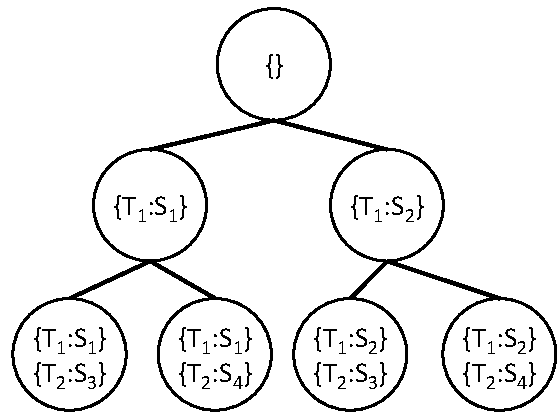
\includegraphics[width=0.6\columnwidth]{search-space-samd_cropped.pdf}
    \caption{An example of part of the \samd search space.}
    \label{fig:search-space}
\end{figure}

% Search space formulation Liat
A graph search problem is defined by a graph $(V,E)$, a start node $s\in V$, and a set of goal nodes $G\subseteq V$, where a solution is a path in the graph from $s$ to a node in $G$.  The graph can be explicitly given as input, or implicitly given by defining an initial node and a set of transition functions that map a node to its neighbors in the graph. 
Branch \& bound (\bnb) is a classic graph search algorithm that includes search space pruning. To use \bnb to solve \samd, we define the following search graph. A node in this graph represents a \emph{partial} supplier assignment function, which is a function that assigns suppliers to a subset of the tasks in $T$. 
The initial node $s$ is the empty supplier assignment function, that is, a partial supplier assignment function that does not assign any supplier to any tasks. 
Every child node of $s$ represents a possible assignment of a supplier to $t_1$. 
Every child node of these nodes represents a possible assignment of a supplier to $t_2$, 
and so forth. Note that this search space is a tree. Figure~\ref{fig:search-space} illustrates two levels of this tree. 
The depth of this tree is the number of tasks $N$, and every leaf node represents a \emph{complete} supplier assignment. 

Searching this tree with \bnb is done as follows. A depth-first search starts with the root of the tree, and progresses until reaching a leaf. We compute the $M$ value for that leaf, and mark it as $M_{best}$. The depth-first search continues, but now we compute the $M$ value for every visited node. If the $M$ value of that node is smaller than $M_{best}$, we prune the subtree rooted by this node, as $M$ values only decrease along a branch in the tree. Whenever a leaf node is reached, we check if its $M$ value is better than $M_{best}$, and update $M_{best}$ if necessary. The search halts when all nodes have been either visited or pruned, at which case $M_{best}$ is optimal. %liat %TAL - many repetitions, so I revised the text

It is easy to see that this implementation of \bnb is complete and optimal. However, its runtime performance may be problematic. This is due to the fact that even for a partial assignment the computation of $M$ must consider the deadline $d$ of the overall project; thus, we suspect that pruning would be rather poor. Nonetheless, the Branch \& Bound approach can still serve as a good baseline.
%Probability to finish before that deadline partial solutions (assignments) have higher values (probabilities) than complete solutions. Thus, pruning can be potentially applied whenever the probability of a partial assignment is already lower than the currently known complete assignment, i.e., the lower bound. However, even for a partial assignment the computation of $M$ must consider the deadline $d$ of the overall project. Therefore, we suspect that pruning would be rather poor, but the Branch \& Bound approach can still serve as a good baseline.
%It is easy to see that this implementation of \bnb is complete and optimal. 

To tackle the above problem, we need to tighten the gap between partial assignments and the deadline of complete assignments. To this end, we propose an optimal algorithm to \samd that is based on the the well-known \astar algorithm~\cite{hart1968formal} with some adjustments. 


% % Goal: optimize the min bound from the approximation
% % Max problem and not a min problem, search on f alone

%\subsection{Solving \samd with A$^*$}
\subsection{Solving \samd with \astar}
\label{sec:astar}


\commentout{
\begin{algorithm}
\small
\KwIn{$\Pi=\tuple{T,S,X,d}$, an \samd problem}
\KwOut{$\varphi$, an optimal supplier assignment}
    $M_{best}\gets 0$; $\varphi_{best}\gets$ null; $\varphi_{init}=\{\}$; \open $\gets \emptyset$\\
    $n_{init}$.task$\gets 0$; $n_{init}$.$\varphi\gets \varphi_{init}$\\
    Add $n_{init}$ to \open with key $U(n_{init})$\\
    \While{\open is not empty}{
        $n_{best}\gets$ pop from \open a node with maximal $U(n)$\\
        \If{$U(n_{best})\leq M_{best}$}{
            \Return $\varphi_{best}$\\
        }
        $i\gets n_{best}$.task\\
        $\varphi\gets n_{best}.\varphi$\\
        \ForEach{supplier $s$ for task $t_{i+1}$}{
            $n_{child}$.task $\gets i+1$\\    $n_{child}.\varphi\gets\varphi\cup(t_i\rightarrow s)$\\
            \eIf{$n_{child}.\varphi$ is a complete assignment}{
                $M\gets M(n_{child})$\\
                \If{$M\geq M_{best}$}{
                    $M_{best}\gets M$\\
                    $\varphi_{best}\gets n_{child}.\varphi$\\
                }
            }{
                Add $n_{child}$ to \open with key $U(n_{child})$\\
            }
        }
    }
    \Return $\varphi_{best}$\\
    \caption{Psuedo-code of \astar for \samd.}
	%\caption{Our \astar-based algorithm for \samd.} 
	\label{alg:astar}
\end{algorithm}
}

% A* Background 
%Next, we propose an \samd algorithm that is based on the well-known \astar algorithm~\cite{hart1968formal} with some adjustments. 
\astar is a best-first search algorithm that maintains two lists of nodes: an open list (termed \open) that contains all nodes that were generated and not expanded yet, and a closed list (termed \closed) that contains all nodes that were already expanded. Initially, \open contains the initial node (in our case, the node representing an empty supplier assignment). Then, in every iteration one node is moved from \open to \closed, and all its children nodes are added to \open. The search halts when a goal node is popped from \open. 

\astar considers two values for every node $n$: 
the cost of the best-known path from the initial node to $n$, 
and a heuristic estimate of the cost of the optimal path from a given node to a goal. 
The former is denoted by $g(n)$ and the latter by $h(n)$. \astar pops from \open in every iteration the 
node with the smallest $g(n)+h(n)$. 
A heuristic $h$ is called \emph{admissible} if its estimate is never larger than the real cost of the optimal path from $n$ to the goal. 
Given an admissible heuristic, \astar is guaranteed to have found the optimal solution when a goal node is expanded. Moreover, under certain conditions, all other algorithms must expand at least the same set of nodes as \astar~\cite{dechter1985generalized,holte2019OnThe}. 


% MAX Problems
Recall that \samd is a \emph{maximization} problem. % because its goal is to find a supplier assignment that maximizes the chance to meet the deadline. 
However, \astar is commonly used for minimization problems, and thus needs some adaptations to the maximization case~\cite{stern2014max}. Two changes are required: (1) an admissible heuristic must return an estimate that is never \emph{smaller than} the real cost to reach a goal, and (2) the search can only halt after the cost of the best solution found so far is larger than or equal to $g(n)+h(n)$ for all $n$ in \open. 

% In our context
To apply \astar as is to solve \samd, we need to define $g(n)$ and $h(n)$. However, 
the notion of paths and costs of paths is not natural in our search space, 
since we can only compute the actual value -- $M(T, \varphi,d)$ -- of a complete supplier assignment. 
Instead of defining $g(n)$ and $h(n)$, we define for every node $n$ a single value, denoted $U(n)$, 
that is an upper bound over the cost of all goal nodes in the subtree of the search space rooted by $n$. 
Then, in every iteration of our modified \astar, we pop from \open the node with the highest $U(n)$ value
and add its children to \open. 
A leaf node represents a complete supplier assignment. So, for every generated leaf node we compute its corresponding $M$ value, and store the leaf with the highest $M$ seen so far. We refer to the supplier assignment of this leaf node as $\varphi_{best}$ and its $M$ value as $M_{best}$.  The search halts when either \open is empty or the expanded node $n$ is such that $U(n)\leq M_{best}$. When the former condition occurs, we know that all supplier assignments have been checked, in which case $\varphi_{best}$ is indeed the optimal supplier assignment. If the latter condition occurs, we know that for all nodes $n\in \open$ it holds that $U(n)\leq M_{best}$, and thus $\varphi_{best}$ is optimal. Consequently, given that an admissible $U(\cdot)$ is implemented, completeness and optimality are guaranteed~\cite{stern2014max,holte2019OnThe}. 

Algorithm~\ref{alg:astar} provides a complete pseudo-code of our \astar-based algorithm. %Liat %TAL - great!
For convenience, for a node $n$ we denote by $n.\varphi$ and $n$.task the partial assignment that $n$ represents and the index of the last task assigned by $n.\varphi$, respectively. Hence, for the initial node $n_{init}$ we have that $n_{init}.\varphi$ is an empty supplier assignment and $n_{init}.$task is zero (line 2 in Algorithm~\ref{alg:astar}). 
Note that due to the tree structure of the search graph, there is no need to maintain \closed.

\begin{algorithm}
\small
\KwIn{$\Pi=\tuple{T,S,X,d}$, an \samd problem}
\KwOut{$\varphi_{best}$, an optimal supplier assignment}
    $M_{best}\gets 0$; $\varphi_{best}\gets$ null; $\varphi_{init}=\{\}$; \open $\gets \emptyset$\\
    $n_{init}$.task$\gets 0$; $n_{init}$.$\varphi\gets \varphi_{init}$\\
    Add $n_{init}$ to \open with key $U'(n_{init})$\\
    \While{\open is not empty}{
        $n\gets$ pop from \open a node with maximal $U'(n)$\\
        \If{$U'(n)\leq M_{best}$}{
            \Return $\varphi_{best}$\\
        }
        $i\gets n$.task\\
        $\varphi\gets n.\varphi$\\
        \ForEach{supplier $s$ for task $t_{i+1}$}{
            $n_{child}$.task $\gets i+1$\\    $n_{child}.\varphi\gets\varphi\cup(t_{i+1}\rightarrow s)$\\
            \eIf{$n_{child}.\varphi$ is a complete assignment}{
                $M\gets M(n_{child})$\\
                \If{$M\geq M_{best}$}{
                    $M_{best}\gets M$\\
                    $\varphi_{best}\gets n_{child}.\varphi$\\
                }
            }{
                Add $n_{child}$ to \open with key $U'(n_{child})$\\
            }
        }
    }
    \Return $\varphi_{best}$\\
    \caption{Psuedo-code of \astar for \samd.}
	%\caption{Our \astar-based algorithm for \samd.} 
	\label{alg:astar}
\end{algorithm}

%\Roni{Do we want a pseudo code??  it is quite easy to do, but somewhat obvious}
%\Roni{Do we want a proof??  it is quite easy to do, but somewhat obvious}\Roni{The text above explains it, not critical to add a proof IMO}

\subsection{Computing an Upper Bound}
\label{sec:ubound}

Our \astar can be used with any implementation of $U(\cdot)$ as long as it %is admissible for maximization problems, i.e., 
returns an upper bound over all the goals in its sub-tree. Next, we propose a concrete admissible $U(\cdot)$ that works well in practice. %We first compute a preliminary heuristic $U'(\cdot)$ from which 

Let $n$ be the node we wish to compute $U(n)$ for, and assume that $n$ represents a partial assignment $\varphi_n$ that assigns a supplier to tasks $t_1,\ldots, t_i$ for some $i<N$. 
We compute $U(n)$ by assuming that in every unassigned task $t\in \{t_{i+1},\ldots,t_{N}\}$ 
all suppliers that can perform this task do so simultaneously, so that the task is completed 
when the fastest one finished. Formally, for the computation of $U(n)$, we assume that the completion time of every unassigned task $t$ is $\min_{s\in S_t} X_s$. This is a random variable that can be computed easily given all the $X_s$ random variables. 
In our setting only a single supplier performs each task, so the real completion time of any single supplier must be greater or equal to this value. This means that by using $\min_{s\in S_t} X_s$ for each unassigned task we \emph{underestimate} the total completion time of the project, thus, \emph{overestimate} the probability of meeting the project deadline. As a consequence, it can serve as an admissible heuristic for the maximization problem at hand.
%Since in our setting only a single supplier performs each task, the real completion time of any single supplier must be larger than this value (or at least equal). Thus, it can be used as an admissible heuristic. 

To summarize, we define $U(n)$ as follows:
\begin{equation}
\small
U(n)=Pr\left(\sum_{t\in \{t_1,\ldots, t_i\}} X_{\varphi_n(t)} + \sum_{t\in \{t_{i+1},\ldots, t_{N}\}} \min_{s\in S_t} X_s\leq d \right)
\label{eq:heuristic}
\end{equation}
% Admissible heuristic

%P(min┬i⁡〖X_i 〗≤a)≥max┬i⁡[P(X_i≤a)]∀a,X
%	Keeping the Admissible Heuristic Polynomial (the one-sided Kolmogorov) – Lemma 4 (one-sided is admissible) and Lemma 5 (this is an optimal approximation given m – from the AAAI 2018 paper)
%Lemma 4 (one-sided is admissible): P(〖OptTrim(X,m)〗⁡〖≤a〗 )≥P(X≤a)  ∀a,X,m

%{Roni{All the above may be too brief and not clear. Maybe we should define a variable for this min variable,a nd then do an $M$ computation on this. Or maybe it is all clear. What do you think?}

% From M to approximation
While the above $U(\cdot)$ is clearly admissible, its computational complexity is equivalent to that of computing the $M$ value of a supplier assignment $\varphi$, which is NP-hard (Theorem~\ref{the:m}). 
%For small problems it may be feasible to apply such a computation for a limited number of times, as is done in \sampling. However, 
$U(n)$ needs to be computed frequently for every node $n$ that is added to \open, which renders its exact computation inapplicable. Hence, we turn to an approximate computation $U'(\cdot)$ of $U(\cdot)$.
%Recall that the problem with computing the $M$ value lies in the exponential growth of the support size \cite{cohen2019estimating}.
%\Roni{Not clear at all. What is ``lies in the exponential growth of the support size''???}
After every addend in the computation of $U(\cdot)$ we apply the \optapprox$(X,m)$ operator \cite{cohen2018optimal}, which for a given random variable $X$ and a requested support size $m$ returns a new random variable $X'$ with a support size of at most $m$ in polynomial time. By restricting the support size to a given $m$ after every addend, we prevent the exponential growth of the support size.

The resulting variable $X'$ of \optapprox$(X,m)$ is actually the best approximation (optimal) of $X$ given the requested support size $m$ according to the ``one-sided'' version of the Kolmogorov distance~\cite{lilliefors1967kolmogorov}. The ``one-sided'' approximation means that the \emph{cumulative distribution function} (CDF) $F_{X'}$ of $X'$ is not smaller than the CDF $F_{X}$ of $X$, i.e., for every value $v$ of $X$, $F_{X}(v)\leq F_{X'}(v)$. This, in turn, results in a \emph{pessimistic} computation of the probability to meet the deadline. However, since \samd is a maximization problem, maintaining admissibility requires an \emph{optimistic} computation. Consequently, we use an \emph{inverse} version of \optapprox that gives $F_{X}(v)\geq F_{X'}(v)$ for all $v$, i.e., an optimistic computation of the probability to meet the deadline. We term the computation of $U(\cdot)$ with inverse \optapprox after every addend as $U'(\cdot)$. 
%\Roni{Instead of the unclear wording of the last sentence, can't we give a formula?}
Clearly, $U'(n)\geq U(n)$ for every $n$. Therefore:

%\Liat{There is a gap between the written heuristic and the implemented one -- regarding the accurate computation of the left addend in Eq.~\ref{eq:heuristic}.}

\begin{comment}
\begin{lemma}
$U'(\cdot)$ is admissible.
\label{lem:admissible}
\end{lemma}

\begin{proof}
$U(\cdot)$ is trivially admissible, since it assumes that all suppliers that can perform a future task will do so simultaneously, which is obviously not worse than any single supplier performing the task. Also, \invoptapprox that is applied in $U'(\cdot)$ is optimistic, hence also admissible.
\end{proof}
\Roni{The above proof doesn't say anything -- it sounds like this:``Our claim is trivially true, because A is trivial and B is trivial, so C is trivial.''. As a reviewer, I'd be mostly annoyed. I recommend removing the proof and the lemma, and just getting to the corrollary.
\end{comment}
\begin{corollary}
\astar for \samd with heuristic $U'$ is complete and optimal.
\end{corollary}

%Note that in order to maintain the optimality of the algorithm we cannot use \optapprox in the computation of $M$ for complete supplier assignments (line 14 in Algorithm~\ref{alg:astar}). Theoretically, this computation is performed an exponential number of times. 
%Nonetheless, in practice our \astar approach manages to refrain from expanding most of the leaves (complete assignments), as is evident from the run-time results of our experimental evaluation (Section~\ref{sec:exp}).

%Note that in all the discussion above, we computed for leaf nodes and for the $U(n)$ computations 
%the exact $M(T,\varphi,d)$ probabilities. Since this is computationally difficult, we can replace it 
%with our poly-time approximation. This will result in our \astar algorithm returning a supplier assignment function that optimizes the approximation. However, we can bound the suboptimality of our \astar by using the approximation bounds of our poly-time approximation. 

\begin{comment}

\section{Finding Approximate Solutions}
\label{sec:approx}

In order to maintain the optimality of the presented \astar algorithm we cannot use \invoptapprox in the computation of $M$ for complete supplier assignments (line 14, Algorithm~\ref{alg:astar}). Theoretically, this computation is performed an exponential number of times, and therefore may limit the scalability of the method. 
\Roni{The term \invoptapprox is not defined anywhere, so the paragraph above makes no sense.}
\Tal{\invoptapprox appeared in Section 3.3, but when we decided to remove Section 4, I also removed it from Section 3.3 (and only used there \optapprox to avoid confusion).}
\Roni{Yeah, I assumed this is the case. But where can I find that text now? I only saw above in a comment that we use \invoptapprox but no definition}
%\Roni{Not clear: when you say we cannot use \invoptapprox, do you mean that if we use it it will be too slow or just incorrect?}
%\Tal{It will be incorrect. There was a space issue, so I tried to be as short as possible. We can definitely add an explanation why using \invoptapprox in line 14 compromises optimality.}Roni: Ok. 

To this end, we propose \astarapprox, an approximate variant of the \astar algorithm that does not compute $M$ and uses an approximation of $M$ instead. 
In particular, \astarapprox uses an approximation of $M$ proposed by Cohen et al~\cite{cohen2015estimating} that we refer to as $M_\epsilon$.  
$M_\epsilon$ accepts a parameter $\epsilon$ and outputs a value 
that is an upper bound on $M$ that is guaranteed to be no more than $\epsilon$ off the real $M$ value.
That is, for every set of tasks $T$, supply assignment $\sigma$, and deadline $d$:
\begin{equation}
    0 \leq M_\epsilon(T,\sigma, d)-M(T,\sigma, d) \leq \epsilon 
    \label{eq:meps}
\end{equation}
\Roni{Liat and Tal: is the above correct?}
\Tal{Almost... The error is one-sided, so it is always optimistic, i.e., you don't need to use the absolute value.
I don't continue to your next comments, because I believe that the absolute value is the source for all the problems including $2\varepsilon$ error instead of $\varepsilon$.}
\Roni{Perfect - TNX! So I changed the inequality above, please verify}

\Roni{I don't know how direct is the computation of $M_\epsilon$ from what you already published. My guess is that in your other paper, you don't talk about $M$, but rather talk more generally about getting an approximation for the sum of random variables. So, here, you need to show how to get from that approximation to an approximation on $M$. In fact, this can be a lemma.}

We denote by $\sigma^*$ be the supplier assignment that maximizes $M$ and $\sigma^*_\epsilon$ be the supplier assignment that maximizes $M_\epsilon$. 
\begin{lemma}
\begin{equation}
    M(\sigma^*) - M(\sigma^*_\epsilon) \leq \epsilon 
\end{equation}
\label{lem:approx}
\end{lemma}
\begin{proof}
By the definitions of $\sigma^*_\epsilon$ and $M_\epsilon$:
\begin{align}
    M_\epsilon(\sigma^*_\epsilon) & \geq M_\epsilon(\sigma^*) \\
    M(\sigma^*_\epsilon)+\epsilon \geq M(\sigma^*) \\
    \epsilon \geq M(\sigma^*)-M(\sigma^*_\epsilon) \\
\end{align}
\end{proof}
The implication of Lemma~\ref{lem:approx} is that a search algorithm that returns the supplier assignment that maximizes $M_\epsilon$ will return a solution to \samd that is at most $\epsilon$ smaller than the optimal solution. 
However, simply replacing $M$ with $M_\epsilon$ in Algorithm~\ref{alg:astar} is not sufficient to guarantee that $\sigma^*_\epsilon$ will be found. 
This is because $U'$ is not an admissible heuristic for optimizing $M_\epsilon$. 

\Roni{MISSING PART1: Here should come an example of why U' is not admissible for this problem.}


To address this, modify our \astar and use a slightly different heuristic. 
We call the modified search algorithm and heuristic \astarapprox and $U'_\epsilon$, respectively. 

\Roni{MISSING PART2: Here should come an explanation of \astarapprox and $U'_\epsilon$, copying from the text below}


To prove that \astarapprox indeed returns $\sigma^*_\epsilon$, we establish the following Lemma. 
\begin{lemma}
For any node $n$ in the search tree of \astarapprox 
it holds that $U'(n)\geq M_\epsilon(n')$ 
for any node $n'$ that is in the subtree rooted by $n$. 
\label{lem:approx-admissible}
\end{lemma}
\begin{proof}
\Roni{MISSING PART4: Must prove this to establish correctness}
\end{proof}

\begin{theorem}
Any solution $\sigma$ returned by \astarapprox satisfies the following:
\begin{equation}
    |M(\sigma)-M(\sigma^*)|\leq 2\epsilon
\end{equation}
\end{theorem}
\begin{proof}
\Roni{One the missing parts above are established, this one is easy and I'm happy to do it.}
\end{proof}

\Roni{Done. Now just need to fill the holes above :)}


The first change shifts the solution space from exact solutions to approximate solutions, by using the \invoptapprox operator even when considering complete assignments. The objective is to find the best solution $M^*_\appr:=\max_\varphi M_\appr(\Pi,\varphi, d)$ within the approximate solutions space. 





%The error of \astarapprox is bounded by $\varepsilon:=\frac{N-1}{m}$.
%\Roni{I assume $N$ is the number of tasks, but who is $m$? I think it's the number of support in your approximation, but it should go the other way around: we set the suboptimality bound, and then choose how many layers you need to get this suboptimality bound}
%\Tal{$m$ is indeed the maximal support size used in the computation. But this is a parameter, so according to the $\varepsilon$ error you want to achieve, you can play with $m$. But what you propose is playing with the number of layers, which seems strange to me, because the number of layers is part of the problem definition, and not a parameter that you can play with.}
%\Roni{No, you mis-understood me. The number of layers is, as you wrote, part of the problem. But $m$, if I understand correctly, is not. So, a user gets $N$ as input, and can choose the $\varepsilon$ that fits the desired suboptimality, and the algorithm needs to then compute $m$. This can turn out much nicely also in terms of writing. We will write a theorem or something like that that says that to obtain suboptimality $\varepsilon$, we need to compute $U_\appr$ with $m=\frac{N-1}{\varepsilon}$.}
%\Tal{I agree. It is indeed better to use $\varepsilon$ as the user's required error parameter, and derive $m$ from it.}

The pseudo-code of \astarapprox extends Algorithm~\ref{alg:astar} with the following required changes:
\begin{enumerate}
    \item Change all computations of $M$ to $M_\appr$ computations, where $M_\appr = \invoptapprox(M)$. \Roni{why do you we need both notations -- $M_\appr$ and $\invoptapprox(M)$ -- if they are the same?}
    \Tal{These are actually not two notations but rather a definition of $M_\appr$, which is applying the \invoptapprox operator on $M$. Perhaps changing '=' to the definition operator ':=' would clarify this.}
    \Roni{No, I suggest just using one. Why do we need two notations? more importantly, \invoptapprox has not been defined yet.}
    \Tal{As stated in a previous comment, \invoptapprox will be re-added to Section 3.3, so at this point it would already be a known concept, with which we could define $M_\varepsilon$.}
    \item Change $U'(\cdot)$ to $U_\appr(\cdot)$ (lines 3, 5, 6 and 19), where $U_\appr(n) = \min (U'(n),U_\appr(n_{parent}))$.
    \item Add $\varepsilon$ to the left side of the inequality of line 6: \\
    \textbf{if} $U_\appr(n)+\varepsilon\leq M_{best}$
\end{enumerate}

The first change shifts the solution space from exact solutions to approximate solutions, by using the \invoptapprox operator even when considering complete assignments. The objective is to find the best solution $M^*_\appr:=\max_\varphi M_\appr(\Pi,\varphi, d)$ within the approximate solutions space. 

The reason for the second change is that $U'(\cdot)$ is no longer admissible when dealing with approximate complete solutions. This is due to the lack of monotonicity of $U'(\cdot)$ in the sense that it does not always hold that $U'(n) \leq U'(n_{parent})$ resulting from the \optapprox error. 
\Roni{The term \emph{monotonicity} should be better defined. Do you mean that $U$ is monotone of for every node $n$ and every child of $n$ $c$, it holds that $U(n)\geq U(c)$?}
\Tal{Indeed. This is why I needed you :-) I was not sure what are the conventions. So we should add a monotonicity definition as you suggested.}
This lack of monotonicity does not impair admissibility of the exact \astar variant, since $U'(n)$ always overestimates the exact $M$ value of every leaf descendant of $n$. However, this does not hold for the $M_\appr$ values that are used in \astarapprox. 

\Roni{So, here is how I suggest to put this:
(1) We define $M_\epsilon$ as an approximation of $M$ that satisfies $|M_\epsilon(\varphi)-M(\varphi)|\leq \epsilon$, for every supplier assignment $\varphi$. 
(2) We define $\varphi^*$ to be the supplier assignment that maximizes $M$, and define $\varphi^*_\epsilon$ to be the supplier assignment that maximizes $M_\epsilon$. 
(3) Lemma 1: For every $\epsilon>0$ it holds that
$M(\varphi^*_\epsilon)+\epsilon\geq M(\varphi^*)$. 
(4) We explain our approach: we modify our \astar so that it finds the supplier assignment that maximizes $M_\epsilon$ instead of $M$. Then, following Lemma 1, we know that its $M$ value is at most $\epsilon$ smaller than the supplier assignment that optimizes $M$.
(5) Explain that simply replacing $M$ with $M\epsilon$ in the pseudo code does not work, because $U_\appr$ is no longer admissible, i.e., there may be a node $n$ that has descendants that has larger $M_\epsilon$ value.
(6) Explain the modified $U_\appr(n)$, that takes the max over the parent's heuristic. Prove that it is indeed always an upper bound on the $M_\epsilon$ value of all of $n$'s descendants.
(7) Now prove that this \astar indeed returns $\varphi^*_\epsilon$. This is, at this stage, trivial. 
Now we can explain the modifications needed to our \astar in order to find $\varphi^*_\epsilon$}
\Tal{I think there are two errors in what you wrote: (1) Lemma 1 should be $M(\varphi^*_\epsilon)\leq M(\varphi^*)+\epsilon$ instead of what you wrote. (2) In your version the definition of $U_\appr(\cdot)$ should be changed to $U_\appr(n) = \min (U'(n)+\varepsilon,U_\appr(n_{parent}))$. The latter change adds $\varepsilon$ to the $U$ values, otherwise correctness is compromised. Now, after the two changes, both options (the one in the paper, and your suggested option) are practically the same -- you either use $U$ values that may be up to $\varepsilon$ smaller than their underlying leaves (and then add the $\varepsilon$ to the termination condition), or add $\varepsilon$ already to $U$ and remove it from the termination condition. It seems to me exactly the same, but your suggestion uses a more classic notion of admissibility, so it is better perhaps. Overall, I like your proposed flow.}

\begin{lemma}
$U_\appr$ is admissible for \astarapprox.
\label{lem:admissibleapprox}
\end{lemma}
\begin{proof}
$U_\appr$ is inherently monotone due to the applied $\min$ operator. Consequently, $U_\appr$ is admissible.
\end{proof}
\Roni{First, you need to define what you mean by admissible for \astarapprox. I guess you want to prove here that 
for every node $n$ and every complete assignment $\varphi$ in the subtree rooted by $n$ it holds that $U_\appr(n)\geq M_\appr(\varphi)$. Can you prove this?}
\Tal{I guess that our above discussion clarifies this issue (just to make sure -- the answer is no. You must add $\varepsilon$ to the left side to make it correct).}


\begin{lemma}
\astarapprox outputs a supplier assignment $\varphi_{best}$ for which $M_\appr(\Pi,\varphi_{best}, d)=M^*_\appr$.
\label{lem:optimalapprox}
\end{lemma}
\begin{proof}
The third change (to line 6) adds $\varepsilon$, the maximal possible error of \optapprox, to the termination condition. 
\Roni{So, the claim here is that 
for every $n$ and every complete assignment $\varphi$ in the subtree rooted by $n$ it holds that $U_\appr(n)+\varepsilon\geq M(\varphi)$? or $U_\appr(n)+\varepsilon\geq M_\appr(\varphi)$?
If we're aiming for finding the assignment with the best $M_\appr$, then we don't want here the added $\varepsilon$.}
\Tal{Indeed, we want the latter (but with $\leq$ in the termination condition, i.e., $U_\appr(n)+\varepsilon\leq M_\appr(\varphi)$. But without adding $\varepsilon$ the condition is not correct, due to the lack of monotonicity in approximated values. So $U_\appr(n)$ may happen to be almost accurate, whereas $M^*_\appr$ may have an error of up to $\varepsilon$, and therefore without adding $\varepsilon$ this may lead to a too early termination condition that overprunes the search space.}
\Roni{(1) You are 100\% right about $\leq$ instead of $\geq$. My bad, sorry!. (2) About the other stuff, we need to talk about this. Either $U_\appr(n)$ is equal to or greater than $M_\appr$ of all the complete assignment under it, in which case we do not need to add $\epsilon$ here, or it doesn't, and then I'm not sure about correctness.}
\Tal{Again, back to the same thing -- I don't think it was wrong (because $\varepsilon$ was added to the termination condition), but with your proposed flow we don't have this issue anymore.}
Thus, the $M$ value for every leaf descendant of node $n$ is not greater than $U_\appr(n)+\varepsilon$, which in turn ensures that $M_{best}$ is maximal upon the activation of the termination condition. This, together with the \astar structure and the admissibility of $U_\appr$ (Lemma~\ref{lem:admissibleapprox}), ensures optimality within the approximate solutions space.
\end{proof}
\begin{theorem}
The error of \astarapprox is bounded by $\varepsilon$.
\label{the:boundapprox}
\end{theorem}
\begin{proof}
Every addition operation with the \optapprox operator has a maximal error of $1/m$~\cite[Lemma 4]{cohen2018optimal}. The computation of $M^*_\appr$ (Lemma~\ref{lem:optimalapprox}) consists of $N$ addends, i.e., $N-1$ addition operations with \optapprox. The error from these additions is cumulative~\cite[Lemma 5]{cohen2019estimating}, and is thus bounded by $\varepsilon=\frac{N-1}{m}$. 
\end{proof}

\end{comment}

\section{Experimental Evaluation}
\label{sec:exp}

Next, we evaluate the performance of the two sub-optimal algorithms -- \sampling and \expectation~-- and the two optimal algorithms -- \bnb and \astar. For \astar we apply the \optapprox operator with a support size of $m=10$. All algorithms were implemented in Python and the experiments were executed on a hardware comprised of an Intel i5-6500 CPU @ 3.20GHz processor and 8GB memory.

\begin{comment}
In order to conduct a more comprehensive evaluation, we also consider two heuristic approaches for the \samd problem -- \sampling and \expectation.
\sampling is an iterative algorithm. In each iteration it \emph{samples} for every supplier $s\in S$ a task completion time $x_s$ according to its distribution $X_s$. This results in a deterministic instance $\Pi_D$ of the \samd problem $\Pi$, due to the now deterministic task completion times of the suppliers. 
Following that, finding the optimal supplier assignment $\varphi$ for $\Pi_D$ is trivial. Finally, the probability that $\varphi$ will meet the deadline in the original \samd problem $\Pi$ is computed by $M(T,\varphi,d)$. This process is repeated for a predefined number of iterations $K$, after which the supplier assignment $\varphi$ that yielded the highest $M$ value is returned. We use $K=100$ iterations hereinafter.

In this section we present two more approaches to solve the \samd problem which are both sub-optimal: \sampling, and \expectation. The \sampling approach we propose samples possible task completion times, generates corresponding ``optimal'' supplier assignments, and chooses the best resulting supplier assignment. We refer to this algorithm as \sampling. \sampling is an iterative algorithm. In every iteration, we sample for every supplier $s\in S$ a possible task completion time $x_s$ according to its distribution $X_s$. 
Then, we create a deterministic \samd problem $\Pi_D$ that has the same set of tasks, suppliers, and deadline as the original problem, and has the deterministic task completion times sampled for every supplier. \sampling accepts a parameter $K$ that indicates the number of iterations that the algorithm will run. Running more iterations of \sampling can never result in returning a worse solution, but consequently increases run time. \Tal{Need to add expectation..}

\expectation considers the \emph{expected} task completion times, and can thus be easily computed in a single iteration. However, \expectation does not consider the given deadline $d$, and can consequently return bad solutions. Loui~\shortcite{loui1983optimal} refers to such a phenomenon as not taking account of ``risk'' (of not meeting the deadline).


In what follows we experimentally evaluate the performance of the four algorithms -- two sub-optimal algorithms, \sampling with 100 samples and \expectation, and two optimal algorithms, the \astar-based algorithm (Subsection~\ref{sec:astar}) and the Branch \& Bound method that was presented in Subsection~\ref{sec:graph}.
As discussed in Subsection~\ref{sec:ubound}, we implement the \astar-based algorithm with $U_{\optapprox}(\cdot)$, due to the computation complexity of computing $U(\cdot)$. In all the experiments we use a support size of $m=10$ for the approximation.

\end{comment}

We compare between the four algorithms in terms of run-time performance and solution quality. For evaluating the solution quality of the sub-optimal methods we refer to the average error, i.e., the difference from the optimal probability to meet a deadline. Obviously, the optimal approaches have no error and always find the optimal solution.  

We considered a range of experimental setups, including synthetic completion-time distributions and distributions extracted from real software projects. 
%The problem instances are in the form of a graph with different number of layers (tasks) and different number of nodes in each layer (suppliers). [[Why introduce new terms: layers and nodes??? why not tasks and suppliers]
We experimented with three deadline types, defined with respect to $d_{max}$, where $d_{max}$ is the worst-case project completion time (excluding the value of failure, see Subsection~\ref{sec:SynthericDist}). % given the maximal values of the distributions of the suppliers (excluding the value of failure, Subsection~\ref{sec:SynthericDist}) and the number of tasks. 
The deadline types are \emph{early} ($0.25{\cdot} d_{max}$), \emph{expected} ($0.5{\cdot} d_{max}$), \emph{late} ($0.75{\cdot} d_{max}$). 
%We use various deadlines in order to examine their effect on the different algorithms, especially on \expectation. Intuitively, we presume that \expectation will perform well for expected deadlines.\roni{Why???}

\subsection{Synthetic Distributions}
\label{sec:SynthericDist}
We consider two types of synthetically generated distributions -- \emph{random}, and \emph{failure}. 
We use a support of size 4 in all the distributions; this is required in order to avoid ``out of memory" errors due to the exponential growth of support sizes when summing random variables~\cite[Lemma~1]{cohen2019estimating}.  
%Due to summation of random variables~\cite[Lemma~1]{cohen2019estimating} we use a support of size 4 to all distributions to keep it in a reasonable size and to avoid ``out of memory" errors.
In the \emph{random distribution} we generate possible completion times for each supplier in the range [0\dots 4] with uniform distribution. The distribution is randomly generated and then normalized to sum up to one.

In the \emph{failure distribution} we uniformly generate a single possible completion time between every two consecutive integers ($0,1,2,3$), except for the last value that is always set to $10^6$. This large value represents a situation in which the supplier can never complete the task, or in other words -- fail. %Indeed, in real-world situations, some suppliers may fail at performing a task. %An example of structural with failure distribution (or \emph{failure} for short) may look like [0.58:0.14, 1.24:0.41, 2.87:0.33, $10^6$:0.12]. 
Note that in our experiments we do not consider normal distribution, since such problems are more easily solved, as the sum of normal distribution can be computed in polynomial time~\cite{schattenberg2005project,olya2014applying}.

%\Roni{It will be nice to have a figure in which we have an example distribution from each type.}

We vary the number of tasks in a project. Due to the obvious limitations of the exponential search space, we used a 10 minute timeout for each instance, which is sufficient to solve problems with up to 8 tasks with \bnb. 
In order to gather significant statistics, we run 20 different problem instances for every configuration of number of tasks, distribution type, and the deadline type. For every task we consider two possible suppliers, each with a different distribution.   

\subsection{Distributions from Software Development}
The next type of distributions we use is to simulate \samd for software projects, in which the suppliers are software developers and the tasks are \emph{user stories} that need to be implemented by a developer. A user story in software development is ``a small piece of functionality of the final software perceived from the end-user point of view''~\cite{rees2002feasible,kassab2015changing}.
%and is one of the most common ways to specify requirements~\cite{kassab2015changing}. 
We extracted information about implemented user stories from three open-source projects: (1) JBoss Developer (\url{https://issues.jboss.org}), (2) Lsst DM (\url{https://jira.lsstcorp.org}), and (3) Spring XD (\url{https://jira.spring.io}). 
Specifically, we extracted the list of user stories that were assigned to a developer and marked as done. For each user story, we extracted the developer assigned to implement it and the number of \emph{sprints} it took to implement this user story. A sprint corresponds to a fixed time frame. Using this data, we created for every developer a distribution of the number of sprints that developer needs to implement a user story. 
In total we obtained the distributions of user story completion time for 39 developers. Here are examples of such completion time distributions: [1:0.95,	2:0.045, 3:0.005] or [1:0.62,	2:0.3,	3:0.07,	4:0.01].
%Figure~\ref{example} shows these distributions for two developers. \Roni{Would be nice to have this figure}
This information is publicly available from JIRA, a popular issue tracking system used by all our projects to manage the development. %See the footnotes for links to this publicly available data. 


With these distributions, we generate two types of \samd problems. 
%The first has 4 tasks (Developer, DM1, DM2, XD), with each task having all the possible developers from the corresponding project's developer pool.We examine the probability to meet the deadline for different deadlines, up to 20 sprints. 
The first type is of randomly generated projects with 4 tasks, where for each task we randomly select (without repetitions) developers from the relevant developer pool. 
We examine how the different number of developers in each task (up to 7 developers) effects the run-time and solution quality. 
In the second type the number of developers is set to 4 for every task, i.e., we randomly select (without repetitions) 4 developers from the relevant developer pool. The parameter we vary here is the number of tasks, up to 7 tasks. We randomly generate 30 instances for each of the latter two problem types.


%\subsection{Results - synthetically-generated distributions}
%\label{sec:resRand}

\subsection{Results: Synthetic Distributions}
\label{sec:res}

Figure~\ref{025rt} plots the run-times of the four algorithms for different numbers of tasks ($x$-axis).
In all conducted experiments, \astar outperforms \bnb in terms of runtime 
for \samd problems instances with 6 or more tasks. \astar is also faster than \sampling, which in most cases returns non-optimal results. The fastest evaluated algorithm is \expectation, however its solution quality is low. For instance, for 6 tasks the average error was $3\cdot 10^{-6}$ for \sampling and $0.004$ for \expectation. For 7 tasks the respective errors are $4 \cdot 10^{-6}$ and $0.002$, and for 8, $5 \cdot 10^{-5}$ and $0.001$.

\commentout{
returning in some cases an error of 1.  
%In other words, \astar guarantees optimality in reasonable run-time. \expectation and \sampling result with an error and do not return the optimal assignment.
For instance, for 6 tasks the average error was $3\cdot 10^{-6}$ for \expectation and $0.004$ for \sampling. For 7 tasks the respective errors are $4 \cdot 10^{-6}$ and $0.002$. %, and for 8 layers they are $4 \cdot 10^{-5}$ and $0.003$. 
}

\begin{figure}[h!]
	\scriptsize	
	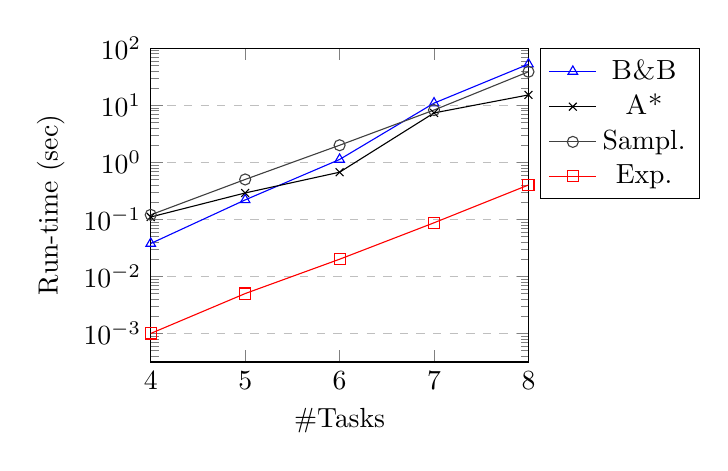
\begin{tikzpicture}
	\begin{axis}[
	scale=0.7,
	ymode=log,
	xlabel={\#Tasks},
	ylabel near ticks,
	ylabel={Run-time (sec)},
	xmin=4, xmax=8,
	ymin=0, ymax=100,
	legend pos=outer north east,
	ymajorgrids=true,
	grid style=dashed,
	]
	
	\addplot[
	color=blue,
	mark=triangle,
	]
	coordinates { 
		(4 , 0.0377) 
		(5 , 0.219) 
		(6 , 1.12)
		(7 , 10.875) 
		(8 , 52.4)

	};
	\addlegendentry{\bnb}
	
	\addplot[
	color=black,
	mark=x,
	]
	coordinates { 
		(4 , 0.11) 
		(5 , 0.29) 
		(6 , 0.67)
		(7 , 7.33) 
		(8 , 15.15)

	};
	\addlegendentry{\astar}
	
	\addplot[
	color=darkgray,
	mark=o,
	]
	coordinates { 
		(4 , 0.12) 
		(5 , 0.5) 
		(6 , 1.988)
		(7 , 8.23) 
		(8 , 38.59)

	};
	\addlegendentry{Sampl.}
	
	\addplot[
	color=red,
	mark=square,
	]
	coordinates {
		(4 , 0.001) 
		(5 , 0.005) 
		(6 , 0.02)
		(7 , 0.087)
		(8 , 0.4)

	};
	\addlegendentry{Exp.}
	
	\end{axis}
	\end{tikzpicture}
	\caption{Run-time comparison of all algorithms for deadline $0.25\cdot maxd$ and random distribution.}\label{025rt}
\end{figure}

\begin{figure}[h!]
	\scriptsize	
	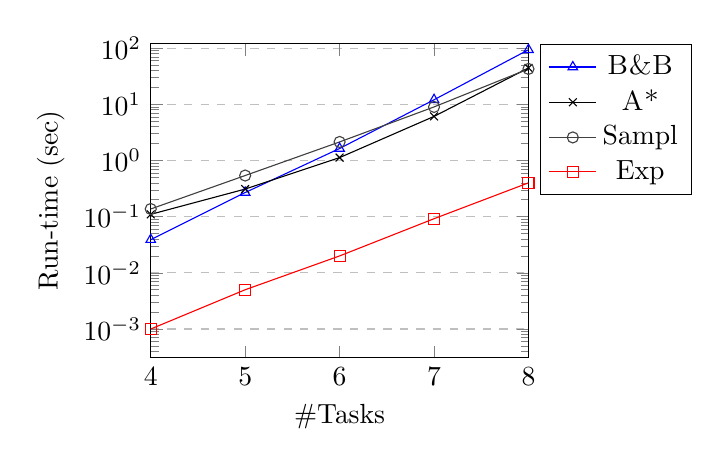
\begin{tikzpicture}
	\begin{axis}[
	scale=0.7,
	ymode=log,
	xlabel={\#Tasks},
	ylabel near ticks,
	ylabel={Run-time (sec)},
	xmin=4, xmax=8,
	ymin=0, ymax=120,
	legend pos=outer north east,
	ymajorgrids=true,
	grid style=dashed,
	]
	
	\addplot[
	color=blue,
	mark=triangle,
	]
	coordinates { 
		(4 , 0.039) 
		(5 , 0.269) 
		(6 , 1.636)
		(7 , 12.058) 
        (8 , 93.77)
	};
	\addlegendentry{\bnb}
	
	\addplot[
	color=black,
	mark=x,
	]
	coordinates { 
		(4 , 0.11) 
		(5 , 0.31) 
		(6 , 1.126)
		(7 , 6.096)
		(8 , 44.46)

	};
	\addlegendentry{\astar}
	
	\addplot[
	color=darkgray,
	mark=o,
	]
	coordinates { 
		(4 , 0.137) 
		(5 , 0.54) 
		(6 , 2.14)
		(7 , 8.99) 
		(8 , 42.7)

	};
	\addlegendentry{Sampl}
	
	\addplot[
	color=red,
	mark=square,
	]
	coordinates {
		(4 , 0.001) 
		(5 , 0.005) 
		(6 , 0.02)
		(7 , 0.092)
		(8 , 0.4)

	};
	\addlegendentry{Exp}
	
	\end{axis}
	\end{tikzpicture}
	\caption{Run-time comparison of all algorithms for deadline $0.75\cdot maxd$ and random distribution.}\label{075rt}
\end{figure}



The low precision of \expectation is illuminated in our experiments with failure distribution. The errors we get when using \expectation are 0.65-0.41, depending on the number of tasks and the deadline; note that such errors are high which is consistent with Example~\ref{exmpl:exp}. 
%\Roni{The text above is out of context. Currently thers no coherent story for the results.}
%We witness such high errors because in many cases the \expectation heuristic algorithm returns that there is no chance to meet the deadline where in fact there is. 
The other algorithms executed with the failure distribution resulted with an error equal to 0. %see Figure~\ref{075faile}. 
In addition, for all other algorithms in this setting  we got 97\%-100\% optimal assignment, but using \expectation we got 0\% optimal assignment for every number of tasks. 
\commentout{
\begin{figure}[h!]
	\scriptsize	
	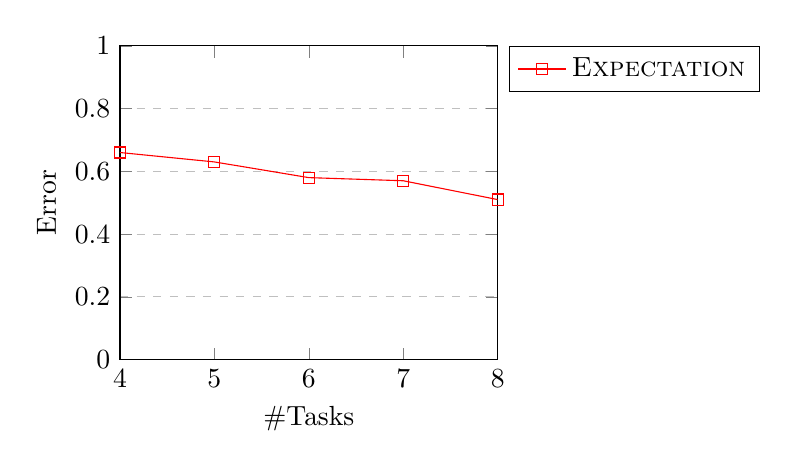
\begin{tikzpicture}
	\begin{axis}[
	scale=0.7,
	xlabel={\#Tasks},
	ylabel near ticks,
	ylabel={Error},
	xmin=4, xmax=8,
	ymin=0, ymax=1,
	legend pos=outer north east,
	ymajorgrids=true,
	grid style=dashed,
	]
	

    \addplot[
	color=red,
	mark=square,
	]
	coordinates {
		(4 , 0.66) 
		(5 , 0.63) 
		(6 , 0.58)
		(7 , 0.57) 
		(8 , 0.51)
		

	};
	\addlegendentry{\expectation}
	
	\end{axis}
	\end{tikzpicture}
	\caption{Error comparison of the heuristic algorithms for deadline $0.75\cdot maxd$ and failure distribution}\label{075faile}
\end{figure}
}
Another concern regarding \expectation is the chosen deadline. As long as the deadline is around the average duration, it is more likely that \expectation will return solid results. However, the deadline is not strict, and in the general case, where the deadline can be very small or very large compared to the expectation, this heuristic may produce substantially sub-optimal results. For a deadline such as $0.5\cdot maxd$ we can observe good results produced by the \expectation heuristic algorithm due to the comfortable deadline. For 4, 5, 6, 7, 8 tasks the results are 93\%, 80\%, 70\%, 90\%, 90\% optimal assignments, respectively.
\commentout{
\begin{figure}[h!]
	\scriptsize	
	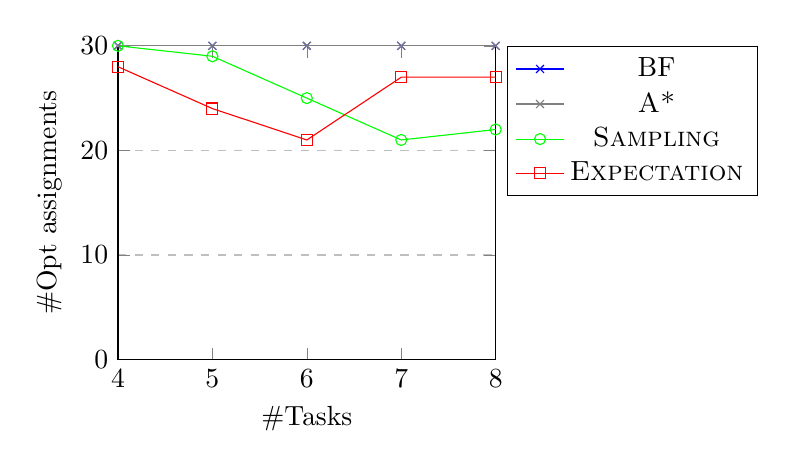
\begin{tikzpicture}
	\begin{axis}[
	scale=0.7,
	xlabel={\#Tasks},
	ylabel near ticks,
	ylabel={\#Opt assignments},
	xmin=4, xmax=8,
	ymin=0, ymax=30,
	legend pos=outer north east,
	ymajorgrids=true,
	grid style=dashed,
	]
	
	\addplot[
	color=blue,
	mark=x,
	]
	coordinates { 
		(4 , 30) 
		(5 , 30) 
		(6 , 30)
		(7 , 30) 
		(8 , 30)
		
	};
	\addlegendentry{BF}
	
	\addplot[
	color=gray,
	mark=x,
	]
	coordinates { 
		(4 , 30) 
		(5 , 30) 
		(6 , 30)
		(7 , 30) 
		(8 , 30)
		
	};
	\addlegendentry{\astar}
	
	\addplot[
	color=green,
	mark=o,
	]
	coordinates { 
		(4 , 30) 
		(5 , 29) 
		(6 , 25)
		(7 , 21) 
        (8 , 22)
	};
	\addlegendentry{\sampling}
	
	
	\addplot[
	color=red,
	mark=square,
	]
	coordinates {
		(4 , 28) 
		(5 , 24) 
		(6 , 21)
		(7 , 27)
		(8 , 27)

	};
	\addlegendentry{\expectation}
	
	
	
	\end{axis}
	\end{tikzpicture}
	\caption{Number of optimal assignments comparison of all heuristic algorithms for deadline of size $0.5\cdot maxd$ and ``Structural" distribution}\label{05reg}
\end{figure}}


We observed that as the number of tasks grows, \sampling is less accurate, even though the error is somewhat small. Because the number of possible assignments grows (exponentially) with the number of tasks, \sampling needs more samples to return good results. Omitted due to space constraints.

The run-time plots in all configuration are mostly similar, and as described before, \astar presents the second best performance in aspect of run-time, see Figures~\ref{025rt} and~\ref{075rt}. 
The best run-time is presented by \expectation, however, the solution quality of this method is poor.

\commentout{
\begin{figure}[h!]
	\scriptsize	
	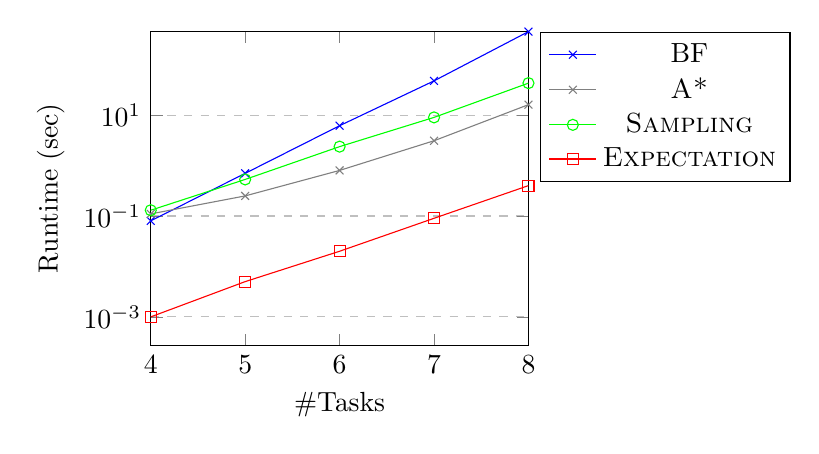
\begin{tikzpicture}
	\begin{axis}[
	scale=0.7,
	ymode = log,
	xlabel={\#Tasks},
	ylabel near ticks,
	ylabel={Runtime (sec)},
	xmin=4, xmax=8,
	ymin=0, ymax=452,
	legend pos=outer north east,
	ymajorgrids=true,
	grid style=dashed,
	]
	
	\addplot[
	color=blue,
	mark=x,
	]
	coordinates { 
		(4 , 0.08) 
		(5 , 0.7) 
		(6 , 6.16)
		(7 , 47.67) 
		(8 , 452) 
		
	};
	\addlegendentry{BF}
	
	\addplot[
	color=gray,
	mark=x,
	]
	coordinates { 
		(4 , 0.11) 
		(5 , 0.25) 
		(6 , 0.8)
		(7 , 3.1) 
		(8 , 16.1)

	};
	\addlegendentry{\astar}
	
	
		\addplot[
	color=green,
	mark=o,
	]
	coordinates { 
		(4 , 0.13) 
		(5 , 0.53) 
		(6 , 2.37)
		(7 , 9) 
		(8 , 43) 
		
	};
	\addlegendentry{\sampling}
	
	\addplot[
	color=red,
	mark=square,
	]
	coordinates {
		(4 , 0.001) 
		(5 , 0.005) 
		(6 , 0.02)
		(7 , 0.09) 
		(8 , 0.4)

	};
	\addlegendentry{\expectation}
	
	\end{axis}
	\end{tikzpicture}
	\caption{Run time comparison of all heuristic algorithms for deadline of size $0.25\cdot maxd$ and ``Failure" distribution}\label{025failrt}
\end{figure}
}

\subsection{Results: Distributions from Software Projects}
%\label{sec:realRes}

Now we report the results of our experiments on the software development distribution types described earlier. 

The first results we present are from the setting where the number of tasks is constant (4 tasks) and the number of possible suppliers to execute the tasks is changed. 

Table~\ref{RealDataNoesDD4Error} shows how the error grows when we add more suppliers, mostly for \sampling. Similarly, the percentage of optimal assignments decreases as we add more optional suppliers. In this setting,  we increase the search space by adding more possible suppliers. The first algorithm to be affected by this is \sampling. As the search space grows, more samples are needed in order to maintain accuracy.
Figure~\ref{RealDataNoesDD4rt} depicts the run-time results for this setting and shows the same trends of the synthetic setting (Figure~\ref{025rt}). Evidently, \bnb takes the longest run-time as the number of developers grows and \expectation takes the shortest run-time (but of course with an error). In the middle of the run-time range are \sampling and \astar, where \astar is optimal and takes shorter run-time as the number of suppliers grows.  

	
\begin{table}
\centering
\resizebox{0.95\columnwidth}{!}{
\begin{tabular}{|l|l|c|c|c|c|c|}
\hline
\multirow{2}{*}{\textbf{}}                                                        & \multirow{2}{*}{\textbf{Algorithm}} & \multicolumn{5}{c|}{\textbf{\#Suppliers}}                       \\ \cline{3-7} 
                                                                                  &                                     & \textbf{3} & \textbf{4} & \textbf{5} & \textbf{6} & \textbf{7} \\ \hline
\multirow{3}{*}{Error}                                                            & \astar/\bnb                                  & 0          & 0          & 0          & 0          & 0          \\ \cline{2-7} 
                                                           
                                                                                  & \sampling                          & 0.017      & 0.047       & 0.063       & 0.094       & 0.097       \\ \cline{2-7} 
                                                                                  & \expectation                         & 0.022      & 0.009      & 0.010      & 0.010      & 0.012       \\ \hline
\multirow{3}{*}{\begin{tabular}[c]{@{}l@{}}\%Opt\end{tabular}} & \astar/\bnb                                  & 100\%         & 100\%         & 100\%         & 100\%         & 100\%         \\ \cline{2-7} 
                           & \sampling                            & 27\%         & 10\%          & 0\%          & 0\%          & 0\%          \\ \cline{2-7} 
                                                                                  & \expectation                         & 20\%          & 27\%          & 13\%          & 17\%          & 13\%          \\ \hline
\end{tabular}
}
\caption{Software projects distributes. Error and percentage of optimal assignments for deadline of 4 sprints and different number of suppliers per task.}\label{RealDataNoesDD4Error}
\end{table}


\commentout{
\begin{figure}[h!]
	\scriptsize	
	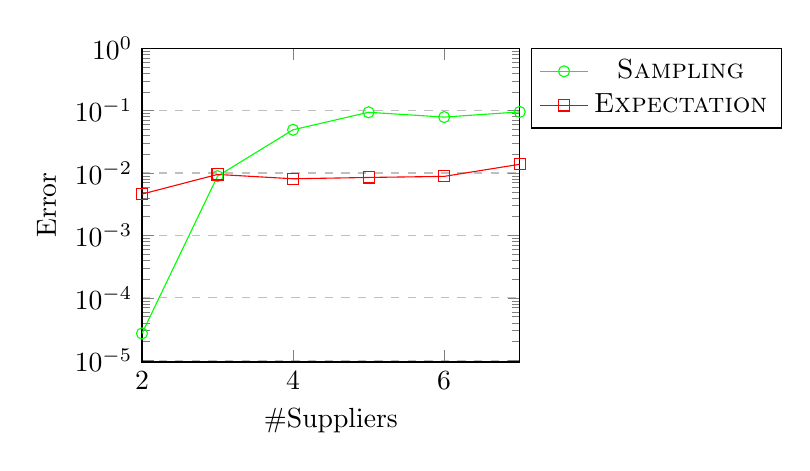
\begin{tikzpicture}
	\begin{axis}[
	scale=0.7,
	ymode = log,
	xlabel={\#Suppliers},
	ylabel near ticks,
	ylabel={Error},
	xmin=2, xmax=7,
	ymin=0, ymax=1,
	legend pos=outer north east,
	ymajorgrids=true,
	grid style=dashed,
	]
	
	
	
	\addplot[
	color=green,
	mark=o,
	]
	coordinates { 
		(2 , 0.000027)
        (3,0.008913301)
        (4, 0.049329392)
        (5, 0.093992466)
        (6,0.078766868)
        (7,0.095318828)
 
		
	};
	\addlegendentry{\sampling}
	
	\addplot[
	color=red,
	mark=square,
	]
	coordinates {
		(2 , 0.0046023)
        (3,0.009501315)
        (4,0.008096098)
        (5,0.008501241)
        (6,0.008842637)
        (7,0.013824363)


	};
	\addlegendentry{\expectation}
	
	\end{axis}
	\end{tikzpicture}
	\caption{Error comparison of all heuristic algorithms for different number of suppliers in each layer, deadline of 4 seconds and real data distribution}\label{RealDataNoesDD4ErrorFig}
\end{figure}

\begin{figure}[h!]
	\scriptsize	
	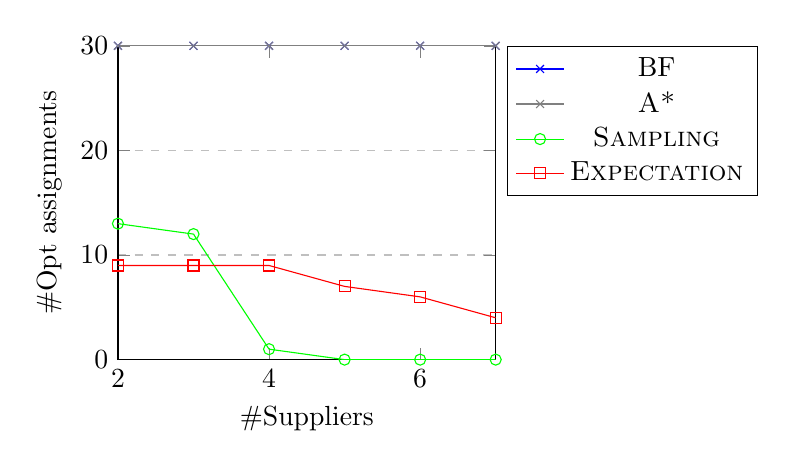
\begin{tikzpicture}
	\begin{axis}[
	scale=0.7,
	xlabel={\#Suppliers},
	ylabel near ticks,
	ylabel={\#Opt assignments},
	xmin=2, xmax=7,
	ymin=0, ymax=30,
	legend pos=outer north east,
	ymajorgrids=true,
	grid style=dashed,
	]
	
	\addplot[
	color=blue,
	mark=x,
	]
	coordinates { 
		(2 , 30) 
		(3 , 30)
		(4 , 30) 
		(5 , 30) 
		(6 , 30)
		(7 , 30) 
		
	};
	\addlegendentry{BF}
	
	\addplot[
	color=gray,
	mark=x,
	]
	coordinates { 
		(2 , 30) 
		(3 , 30)
		(4 , 30) 
		(5 , 30) 
		(6 , 30)
		(7 , 30) 

	};
	\addlegendentry{\astar}
	
	
		\addplot[
	color=green,
	mark=o,
	]
	coordinates { 
		(2 , 13) 
		(3 , 12)
		(4 , 1) 
		(5 , 0) 
		(6 , 0)
		(7 , 0) 
		
	};
	\addlegendentry{\sampling}
	
	\addplot[
	color=red,
	mark=square,
	]
	coordinates {
		(2 , 9) 
		(3 , 9)
		(4 , 9) 
		(5 , 7) 
		(6 , 6)
		(7 , 4)

	};
	\addlegendentry{\expectation}
	
	\end{axis}
	\end{tikzpicture}
	\caption{Number of optimal assignments comparison of all heuristic algorithms for different number of suppliers in each layer, deadline of 4 seconds and real data distribution}\label{RealDataNoesDD4ErrorFig}
\end{figure}
}

%The following experimental settings are with different number of layers (tasks), as shown in Section~\ref{sec:resRand} but here with real application data. 
Finally, we vary the number of tasks. %Table~\ref{RealDataNoesDD4ErrorLayers} presents the error and percentage of optimal assignments results for this setting.
The error results are in the range 0.04-0.052 for \sampling and in the range 0.007-0.01 for \expectation. These algorithms return an optimal assignment in only a small fraction of the case: less than 7\% for \sampling and between 10\% and 33\% for \expectation. In software projects, the distributions behave in a sense that short execution times come with high probabilities. We conjecture that the presented results are highly affected by the shape of the probability distribution. 
The expected completion time for the real project distribution gives very low weight to long execution time, therefore, most suppliers have similar expectations. Regarding \sampling, we observed that due to the shape of the probability distribution most samples indicated a short execution time such that the project will meet the deadline with high probability, which is not true when taking into account the real, full, data. 

As shown in Figure~\ref{RealDataNoesDD4RT}, the run-time in this case behaves a bit differently. We observe that the run-time of \sampling is shorter than that of \astar. However, as already discussed, the solution quality of \sampling in this case is poor. 

\begin{figure}[h!]
	\scriptsize	
	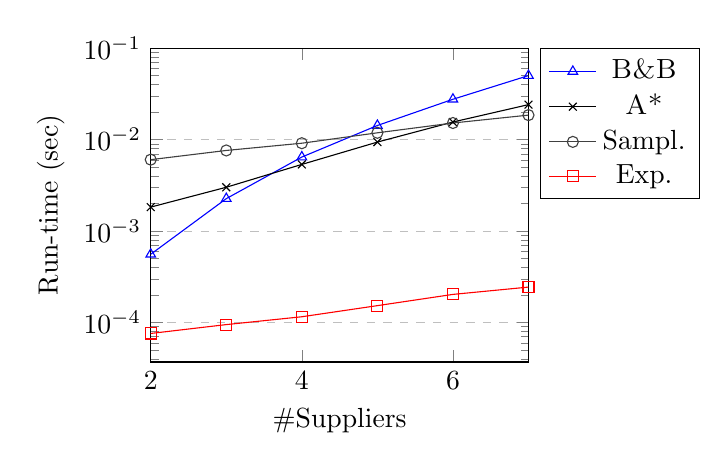
\begin{tikzpicture}
	\begin{axis}[
	scale=0.7,
	ymode = log,
	xlabel={\#Suppliers},
	ylabel near ticks,
	ylabel={Run-time (sec) },
	xmin=2, xmax=7,
	ymin=0, ymax=0.1,
	legend pos=outer north east,
	ymajorgrids=true,
	grid style=dashed,
	]
	
	\addplot[
	color=blue,
	mark=triangle,
	]
	coordinates { 
		(2 , 0.000557844)
        (3, 0.002263546)
        (4,0.006449771)
        (5,0.014273604)
        (6,0.027623041)
        (7,0.050131249)
	};
	\addlegendentry{\bnb}
	
	\addplot[
	color=black,
	mark=x,
	]
	coordinates { 
		(2 , 0.001829243)
        (3,0.00301431)
        (4,0.005357965)
        (5,0.009398643)
        (6,0.015578524)
        (7,0.024137712)


	};
	\addlegendentry{\astar}
	
	
	\addplot[
	color=darkgray,
	mark=o,
	]
	coordinates { 
		(2 , 0.006039135)
        (3,0.007614748)
        (4,0.009136232)
        (5,0.01187253)
        (6,0.015196522)
        (7,0.018537887)

		
	};
	\addlegendentry{Sampl.}
	
	\addplot[
	color=red,
	mark=square,
	]
	coordinates {
		(2 , 0.000076)
        (3,0.000095)
        (4,0.000115705)
        (5,0.000153089)
        (6,0.000203149)
        (7,0.000244196)
	};
	\addlegendentry{Exp.}
	
	\end{axis}
	\end{tikzpicture}
	\caption{Run-time comparison of all algorithms for different number of suppliers in each layer, deadline of 4 sprints and real data distribution.}
	\label{RealDataNoesDD4rt}
\end{figure}
\commentout{
\begin{table}
\centering
\resizebox{0.95\columnwidth}{!}{
\begin{tabular}{|l|l|l|l|l|l|l|}
\hline
\multirow{2}{*}{\textbf{}}                                                        & \multirow{2}{*}{\textbf{Alg.}} & \multicolumn{5}{c|}{\textbf{\#Tasks}}                       \\ \cline{3-7} 
                                                                                  &                                     & \textbf{3} & \textbf{4} & \textbf{5} & \textbf{6} & \textbf{7} \\ \hline
\multirow{3}{*}{Error}                                                            & \astar/BF                                  & 0          & 0          & 0          & 0          & 0          \\ \cline{2-7} 
                                                           
                                                                                  & Sampl.                          & 0.046      & 0.048       & 0.039       & 0.046       & 0.052       \\ \cline{2-7} 
                                                                                  & Exp.                         & 0.01      & 0.009      & 0.009      & 0.009      & 0.007       \\ \hline
\multirow{3}{*}{\begin{tabular}[c]{@{}l@{}}\#Opt\end{tabular}} & \astar/BF                                  & 100\%         & 100\%         & 100\%         & 100\%         & 100\%         \\ \cline{2-7} 
                           & Sampl.                            & 7\%         & 7\%          & 0\%          & 0\%          & 0\%          \\ \cline{2-7} 
                                                                                  & Exp.                         & 17\%          & 33\%          & 20\%          & 10\%          & 17\%          \\ \hline
\end{tabular}
}
\caption{Error and percentage of optimal assignments comparison of all algorithms for different number of tasks, deadline of $0.25\cdot maxd$ sprints and real data distribution}\label{RealDataNoesDD4ErrorLayers}
\end{table}
}







\begin{figure}[h!]
	\scriptsize	
	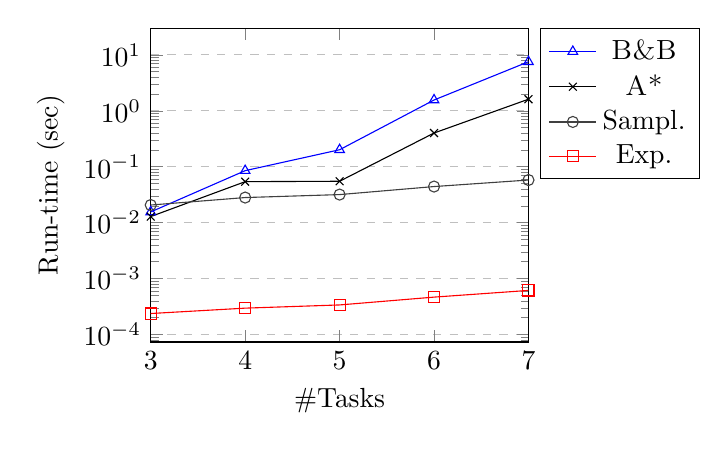
\begin{tikzpicture}
	\begin{axis}[
	scale=0.7,
	ymode = log,
	xlabel={\#Tasks},
	ylabel near ticks,
	ylabel={Run-time (sec) },
	xmin=3, xmax=7,
	ymin=0, ymax=30,
	legend pos=outer north east,
	ymajorgrids=true,
	grid style=dashed,
	]
	
	\addplot[
	color=blue,
	mark=triangle,
	]
	coordinates { 
        (3, 0.015565864)
        (4,0.085139457)
        (5,0.201444316)
        (6,1.561145123)
        (7,7.544835583)

	};
	\addlegendentry{\bnb}
	
	\addplot[
	color=black,
	mark=x,
	]
	coordinates { 
        (3,0.012866235)
        (4,0.054131158)
        (5,0.055021803)
        (6,0.400940522)
        (7,1.613446736)



	};
	\addlegendentry{\astar}
	
	
		\addplot[
	color=darkgray,
	mark=o,
	]
	coordinates { 
        (3,0.020679792)
        (4,0.028132216)
        (5,0.031788397)
        (6,0.044241222)
        (7,0.057902042)


		
	};
	\addlegendentry{Sampl.}
	
	\addplot[
	color=red,
	mark=square,
	]
	coordinates {
        (3,0.000237433)
        (4,0.000296291)
        (5,0.000338062)
        (6,0.000466474)
        (7,0.000614365)

	};
	\addlegendentry{Exp.}
	
	\end{axis}
	\end{tikzpicture}
	\caption{Run-time comparison of all algorithms for different number of tasks, deadline of $0.25\cdot maxd$ sprints and real data distribution.}\label{RealDataNoesDD4RT}
\end{figure}






\commentout{
\begin{figure}[h!]
	\scriptsize	
	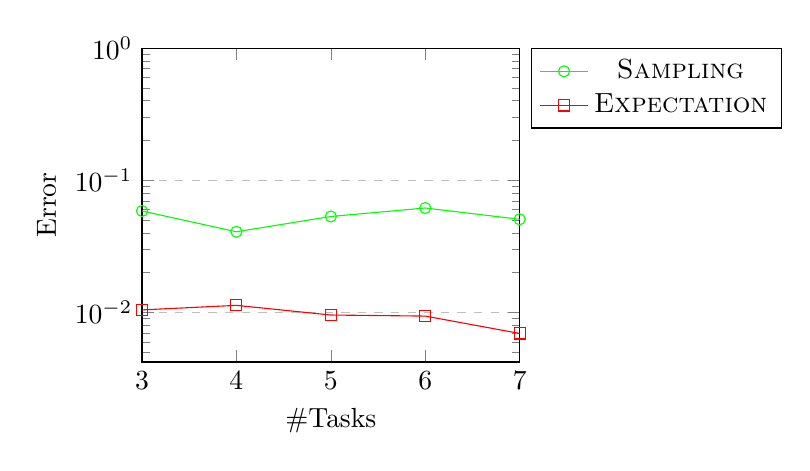
\begin{tikzpicture}
	\begin{axis}[
	scale=0.7,
	ymode = log,
	xlabel={\#Tasks},
	ylabel near ticks,
	ylabel={Error},
	xmin=3, xmax=7,
	ymin=0, ymax=1,
	legend pos=outer north east,
	ymajorgrids=true,
	grid style=dashed,
	]
	
	

	
	\addplot[
	color=green,
	mark=o,
	]
	coordinates { 
        (3,0.058648406)
        (4,0.040836635)
        (5,0.053282065)
        (6,0.061770479)
        (7,0.05073542)
        

 
		
	};
	\addlegendentry{\sampling}
	
	\addplot[
	color=red,
	mark=square,
	]
	coordinates {
        (3,0.010470007)
        (4,0.01132907)
        (5,0.009574956)
        (6,0.009398957)
        (7,0.006946578)



	};
	\addlegendentry{\expectation}
	
	\end{axis}
	\end{tikzpicture}
	\caption{Error comparison of all heuristic algorithms for different number of tasks, deadline of $0.25\cdot maxd$ seconds and real data distribution}\label{RealDataNoesDD4Error25}
\end{figure}

\begin{figure}[h!]
	\scriptsize	
	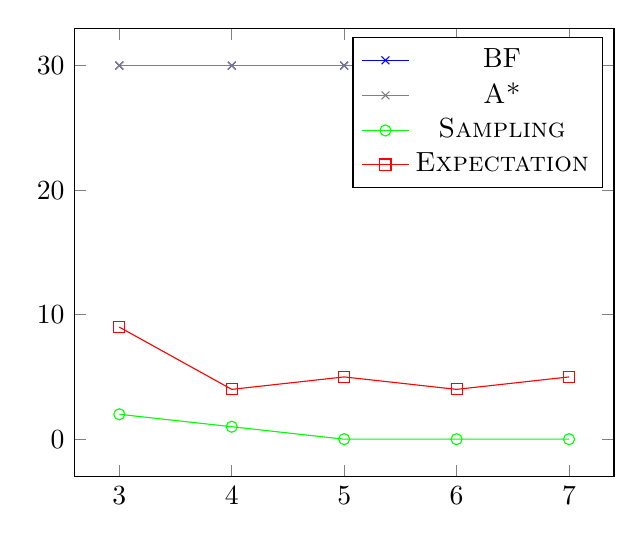
\begin{tikzpicture}
	\begin{axis}
	scale=0.7,
	xlabel={\#Tasks},
	ylabel near ticks,
	ylabel={\#Opt assignments},
	xmin=3, xmax=7,
	ymin=0, ymax=30,
	legend pos=outer north east,
	ymajorgrids=true,
	grid style=dashed,
	]
	
	\addplot[
	color=blue,
	mark=x,
	]
	coordinates { 
		(3 , 30)
		(4 , 30) 
		(5 , 30) 
		(6 , 30)
		(7 , 30) 
		
	};
	\addlegendentry{BF}
	
	\addplot[
	color=gray,
	mark=x,
	]
	coordinates { 
		(3 , 30)
		(4 , 30) 
		(5 , 30) 
		(6 , 30)
		(7 , 30) 

	};
	\addlegendentry{\astar}
	
	
		\addplot[
	color=green,
	mark=o,
	]
	coordinates { 
		(3 , 2)
		(4 , 1) 
		(5 , 0) 
		(6 , 0)
		(7 , 0) 
		
	};
	\addlegendentry{\sampling}
	
	\addplot[
	color=red,
	mark=square,
	]
	coordinates {
		(3 , 9)
		(4 , 4) 
		(5 , 5) 
		(6 , 4)
		(7 , 5)

	};
	\addlegendentry{\expectation}
	
	\end{axis}
	\end{tikzpicture}
	\caption{Number of optimal assignments comparison of all heuristic algorithms for different number of tasks, deadline of $0.25\cdot maxd$ seconds and real data distribution}\label{RealDataNoesDD4Ass}
\end{figure}



}
%-------------------------------All combinations results ----------------------------------------





%Describe: 
%a tree and the distributions
%what is layer
%example of tree
%dijkstra
%sampling


%4.	Dijkstra-based Heuristics
%o	Preliminaries on why Dijkstra cannot work on the CDFs (this may move to Section 2)
%o	Heuristic based on mean time
%o	Heuristic based on highest probability in shortest time
%o	Using sampling, create a deterministic problem, find the path by Dijkstra and approximate the success probability of this path by one-sided Kolmogorov (and resample 100 or 10,000 times and choose the best path).
%5.	Experimental evaluation
%o	Optional: On small problems, comparing all options (from Sections 3 and 4) to the optimal (exact) solution 
%o	On small problems, comparing between the exact solution, full A*, and partial A* (with min heuristic, but without one-sided Kolmogorov)
%o	On large problems, comparing our A* to the option from Section 4

	%Optional: On small problems, comparing all options (from Sections 3 and 4) to the optimal (exact) solution  	On small problems, comparing between the exact solution, full A*, and partial A* (with min heuristic, but without one-sided Kolmogorov) 	On large problems, comparing our A* to the option from Section 4  	Conclusions

\section{Approaches to Scale to Larger Problems}
\label{sec:scale}

As shown in the previous section, the scalability of the optimal algorithms is rather limited. Nevertheless, there are several natural extensions to our work that can increase scalability to larger \samd problems.
\begin{itemize}
    \item \textbf{Task-ordering heuristics.} In our search tree, the tasks were ordered in an arbitrary, fixed, manner. One may create task-ordering heuristic to try to prune partial assignments faster. 
    \item \textbf{\optapprox instead of $M$ for complete assignments.} 
    The computational complexity of computing $M$ values (Theorem~\ref{the:m}) is a clear bottleneck to all algorithms. Instead, one may use \optapprox to approximate $M$ for complete supplier assignments (line 14, Algorithm~\ref{alg:astar}). 
\end{itemize}

The latter approach may ensure that the error is \emph{bounded} in all solutions returned~\cite{cohen2018optimal}, thereby introducing a tradeoff between solution quality and runtime. Note that turning to approximate solutions is not trivial, since $U'(n)$ is no longer an admissible approximation of solutions in the tree rooted by $n$.  This is due to the lack of monotonicity of $U'(\cdot)$ in the sense that it does not always hold that $U'(n) \leq U'(n_{parent})$ resulting from the \optapprox error. This lack of monotonicity does not impair admissibility of the exact \astar variant, since $U'(n)$ always overestimates the exact $M$ value of every leaf descendant of $n$. However, this does not hold for the $M$ values that are used in the approximate \astar variant. To this end, monotonicity can be enforced by switching to an alternative admissible heuristic $U_\appr(n) = \min (U'(n),U_\appr(n_{parent}))$. Also, the error of \optapprox should be considered in the termination condition to ensure completeness (within the approximate solutions space).

%However, these limits can be stretched to some extent by applying task-ordering heuristics. Such heuristics seem especially appropriate in \samd due to the \emph{commutativity} of addition operations.\Roni{I understand what you are saying, but I don't think an average reviewer that did not think about this problem before, will. Recommended change: ".... these limits can be stretched to some extent by applying task-ordering heuristics, i.e., by choosing which task to assign a supplier to first during the search.''}


%The use of \optapprox ensures that the error is \emph{bounded} in all considered approximate solutions~\cite{cohen2018optimal}. However, turning to approximate solutions is not trivial, since $U'(\cdot)$ is no longer admissible in the approximate solutions space. This is due to the lack of monotonicity of $U'(\cdot)$ in the sense that it does not always hold that $U'(n) \leq U'(n_{parent})$ resulting from the \optapprox error. This lack of monotonicity does not impair admissibility of the exact \astar variant, since $U'(n)$ always overestimates the exact $M$ value of every leaf descendant of $n$. However, this does not hold for the $M$ values that are used in the approximate \astar variant. To this end, monotonicity can be enforced by switching to an alternative admissible heuristic $U_\appr(n) = \min (U'(n),U_\appr(n_{parent}))$. Also, the error of \optapprox should be considered in the termination condition to ensure completeness (within the approximate solutions space).

\begin{comment}

%The computational complexity of computing $M$ values (Corollary~\ref{cor:m}) inherently limits the scalability of the complete algorithms, as shown in the previous section. However, these limits can be stretched to some extent by applying task-ordering heuristics. Such heuristics seem especially appropriate in \samd due to the \emph{commutativity} of addition operations.
%Another approach that may lead to considerably better scalability is to use \invoptapprox also in the computation of $M$ for complete supplier assignments (line 14, Algorithm~\ref{alg:astar}). By doing that, the algorithm 
%In order to maintain the optimality of the presented \astar algorithm we cannot use \invoptapprox in the computation of $M$ for complete supplier assignments (line 14, Algorithm~\ref{alg:astar}). Theoretically, this computation is performed an exponential number of times, and therefore may limit the scalability of the method. 

To this end, we propose \astarapprox, an approximate variant of the \astar algorithm, which uses \invoptapprox also for complete supplier assignments. The error of \astarapprox is bounded by $\varepsilon:=\frac{N-1}{m}$.

The pseudo-code of \astarapprox extends Algorithm~\ref{alg:astar} with the following required changes:
\begin{enumerate}
    \item Change all computations of $M$ to $M_\appr$ computations, where $M_\appr = \invoptapprox(M)$.
    \item Change $U'(\cdot)$ to $U_\appr(\cdot)$ (lines 3, 5, 6 and 19), where $U_\appr(n) = \min (U'(n),U_\appr(n_{parent}))$.
    \item Add $\varepsilon$ to the left side of the inequality of line 6: \\
    \textbf{if} $U_\appr(n)+\varepsilon\leq M_{best}$
\end{enumerate}

The first change shifts the solution space from exact solutions (complete assignments) to approximate solutions, by using the \invoptapprox operator even when considering complete assignments. The objective is to find the best solution $M^*_\appr:=\max_\varphi M_\appr(\Pi,\varphi, d)$ within the approximate solutions space. 

The reason for the second change is that $U'(\cdot)$ is no longer admissible when dealing with approximate complete solutions. This is due to the lack of monotonicity of $U'(\cdot)$ in the sense that it does not always hold that $U'(n) \leq U'(n_{parent})$ resulting from the \optapprox error. This lack of monotonicity does not impair admissibility of the exact \astar variant, since $U'(n)$ always overestimates the exact $M$ value of every leaf descendant of $n$. However, this does not hold for the $M_\appr$ values that are used in \astarapprox. 

\begin{lemma}
$U_\appr$ is admissible for \astarapprox.
\label{lem:admissibleapprox}
\end{lemma}
\begin{proof}
$U_\appr$ is inherently monotone due to the applied $\min$ operator. Consequently, $U_\appr$ is admissible.
\end{proof}

\begin{lemma}
\astarapprox outputs a supplier assignment $\varphi_{best}$ for which $M_\appr(\Pi,\varphi_{best}, d)=M^*_\appr$.
\label{lem:optimalapprox}
\end{lemma}
\begin{proof}
The third change (to line 6) adds $\varepsilon$, the maximal possible error of \optapprox, to the termination condition. Thus, the $M$ value for every leaf descendant of node $n$ is not greater than $U_\appr(n)+\varepsilon$, which in turn ensures that $M_{best}$ is maximal upon the activation of the termination condition. This, together with the \astar structure and the admissibility of $U_\appr$ (Lemma~\ref{lem:admissibleapprox}), ensures optimality within the approximate solutions space.
\end{proof}
\begin{theorem}
The error of \astarapprox is bounded by $\varepsilon$.
\label{the:boundapprox}
\end{theorem}
\begin{proof}
Every addition operation with the \optapprox operator has a maximal error of $1/m$~\cite[Lemma 4]{cohen2018optimal}. The computation of $M^*_\appr$ (Lemma~\ref{lem:optimalapprox}) consists of $N$ addends, i.e., $N-1$ addition operations with \optapprox. The error from these additions is cumulative~\cite[Lemma 5]{cohen2019estimating}, and is thus bounded by $\varepsilon=\frac{N-1}{m}$. 
\end{proof}

\end{comment}

\section{Conclusion and Future Work}
\label{sec:conc}

We introduced the \samd problem of assigning suppliers to tasks so as to maximize the probability to meet a given project deadline. For the purpose of solving this problem we proposed two simple suboptimal algorithms and two optimal algorithms, including an optimal \astar-based algorithm that constitutes the highlight of our work.
%for solving this problem. %, as well as a bounded approximation variant, \astarapprox.
%Several algorithms were proposed. Two suboptimal algorithms, \sampling and \expectation, and an optimal \astar-based algorithm that constitutes the highlight of our work.

% The focus on heuristic methods and on an \astar-based approach is due to our conjecture that \samd is a computationally hard problem. Indeed, we showed in Section~\ref{sec:def} that even assessing the probability of meeting the deadline for a single supplier assignment is already NP-hard (Corollary~\ref{cor:m}). Furthermore, we suspect that solving \samd is even harder, since it involves traversing a potentially exponential solution space of such supplier assignments. In Section~\ref{sec:graph} we presented a natural search space for \samd. As we proceed to show, given that search space, the \samd problem does not have the \emph{optimal substructure} property~\cite{cormen2009introduction}. %which is important for applying efficient dynamic programming.
% Consider the example from Section~\ref{sec:def} with the deadline 2, i.e., the \samd problem problem $\Pi=\langle T, S, X, 2\rangle$. The optimal supplier assignment for this problem is $\varphi_{2,4}$. Now, consider a reduced problem $\Pi'$ that consists of only the first task with $T'=\{T_1\}$, $S'=\{s_1,s_2\}$, and the task completion distributions $X'$, which are equal to those of $X$ for the suppliers of the reduced problem. The optimal supplier assignment for $\Pi'=\langle T', S', X', 2\rangle$ is $\varphi_{1}$ for which $M(T',\varphi_{1}, 2)=1$. Obviously, supplier $s_1$ that constitutes the optimal assignment for the first task $T_1$ is not part of the optimal assignment of the extended two-task problem $\Pi$, hence partial supplier assignments in \samd are not necessarily optimal substructures. 
% The absence of optimal substructures prevents the use of efficient dynamic programming approaches (cf. the \emph{relax} operation when solving the shortest path problem~\cite{bellman1958routing,dijkstra1959note}). This observation, together with Corollary~\ref{cor:m}, leads to our main conjecture that the \samd problem is NP-hard. The proof is left open for future research.
Experimental evaluation on synthetic data as well as data collected from real software projects showed promising trends for our \astar algorithm finds, in general, better solutions than the suboptimal algorithms, and on the other hand, outperforms a \bnb implementation in terms of run-time as problems get harder. %Moreover, the bounded approximation variant achieves much-improved scalability.
%In future work we plan to explore task-ordering heuristics, which seem appropriate in \samd due to the \emph{commutativity} of addition operations.
We believe that the presented \samd problem is a challenging problem that can bridge the gap between the research areas of Artificial Intelligence and Project Management. In future research it will also be interesting to see how \samd can be extended to accommodate common features of many real-world projects, such as the inclusion of parallel tasks and online settings~\cite{hentenryck2009online}.
Another direction for future work is to study the task-ordering heuristics and the bounded approximation \astar variant that were proposed in Section~\ref{sec:scale}.

%In addition, as shown in the previous section, the scalability of the proposed optimal algorithms (\bnb and \astar) is rather limited. However, these limits can be stretched to some extent by applying \emph{task-ordering} heuristics. Such heuristics seem especially appropriate in \samd due to the \emph{commutativity} of addition operations. In addition, one may aim for returning solutions that are bounded-suboptimal, trading off optimality for computational efficiency. 

%For future work, one may consider using approximations of computations of $M(\cdot)$. 
%This will compromise the optimality of the algorithm, but will enable using the (now suboptimal) \astar-based approach to much larger problems.



% Nevertheless, its exponential search space prevents applying it to large-scale projects. One of the main barriers in this context is the exact computation of $M$ for complete supplier assignments (line 14 in Algorithm~\ref{alg:astar}). An interesting direction for future work would be to use \optapprox also there (instead of only in the computation of $U_{\optapprox}(\cdot)$). This, in turn, will of course compromise the optimality of the algorithm, but will enable using the (now suboptimal) \astar-based approach to much larger problems.

%\subsubsection*{Acknowledgements}
%Use unnumbered third level headings for the acknowledgements title. All acknowledgements go at the end of the paper.

%\newpage
%\bibliographystyle{aaai21}
\bibliography{ijcai19}

\end{document}
%better examples